\documentclass[8pt]{beamer}
\usepackage{tikz}
\usepackage[utf8]{vietnam}
\usepackage{amsmath}
\usepackage{graphicx}
\usepackage{wrapfig}
\usepackage{hyperref}
\usepackage{mathrsfs}
\usepackage{verbatim}
\usepackage{algorithm}
\usepackage{algpseudocode}
\usetheme{Copenhagen}
\usecolortheme{dolphin}
\setbeamertemplate{navigation symbols}{}
\setbeamertemplate{headline}{}
\title[Chương 4: Thiết kế bộ lọc IIR] %optional
{Chương 4: Thiết kế bộ lọc IIR}
\subtitle{Xử lý tín hiệu số}
\author[Xử lý tín hiệu số] % (optional)
{Tín Vũ}
\date[VLC 2021] % (optional)
{tinvu1309@gmail.com}
\begin{document}
\frame{\titlepage}
\begin{frame}{Mục lục}
\tableofcontents
\end{frame}
\begin{frame}{Giới thiệu playlist}
\section{Giới thiệu playlist}
	\begin{itemize}
		\item Mình là Tín Vũ, hiện đang là sinh viên học tại Trường Đại học Công nghệ, Đại học Quốc gia Hà Nội. Mình tạo playlist video này để hỗ trợ các bạn học môn \textbf{Xử lý tín hiệu số}.
\item Khác với môn học tiên quyết \alert{Tín hiệu hệ thống} trước đó, bài giảng môn học này \textbf{hoàn toàn bám sát với đề cương và giáo trình nội bộ} của trường mình, nên các bạn trường khác cần phải lưu ý rất kĩ điều này.
\item Không chỉ dừng lại ở lý thuyết, playlist này \textbf{có bổ sung hướng dẫn lập trình cơ bản bằng GNU Octave/Matlab} để vẽ phổ tín hiệu, đáp ứng tần số và thiết kế bộ lọc.
\item Môn học này bao gồm \textbf{6 chương}, các chương đều liên quan rất chặt chẽ với nhau nên hãy học cẩn thận ngay từ \alert{Chương 0} để ôn thi cuối kì đỡ vất vả.
	\end{itemize}
\end{frame}
\begin{frame}{Tài liệu tham khảo}
\section{Tài liệu tham khảo}
\begin{itemize}
		\item Tài liệu tham khảo chính: Giáo trình Xử lý tín hiệu số (Nguyễn Linh Trung, Trần Đức Tân, Huỳnh Hữu Tuệ, ĐHCN, 2012).
		\item Tài liệu tham khảo phụ: Discrete-time Signal Processing (Alan V.Oppenheim, 2nd edition). 
	\end{itemize}
\end{frame}
\begin{frame}{Quy trình xử lý tín hiệu số}
\section{Quy trình xử lý tín hiệu số}
\begin{figure}[h]
			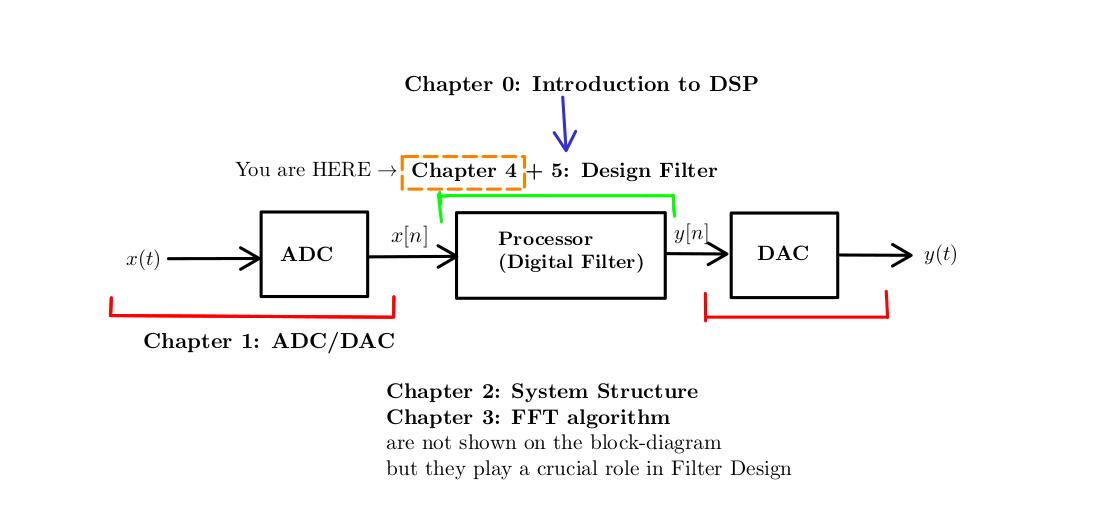
\includegraphics[width=1.1\textwidth]{1.jpg}
			\caption{DSP Learning Process}			\label{fig:re1}
		\end{figure}

\end{frame}
\begin{frame}{Thiết kế bộ lọc tương tự}
\section{Thiết kế bộ lọc tương tự}
\begin{itemize}
	\item Ý tưởng thiết kế bộ lọc tương tự 
\end{itemize}
\subsection{Ý tưởng thiết kế bộ lọc tương tự}
\subsubsection{Bộ lọc thông thấp (LP)}
\begin{itemize}
\item[-] Bộ lọc thông thấp (LP)
\end{itemize}
Ta bắt đầu khảo sát từ sơ đồ mạch của bộ lọc thông thấp (lowpass filter - LP) bậc 1 đơn giản nhất:
\begin{figure}[h]
			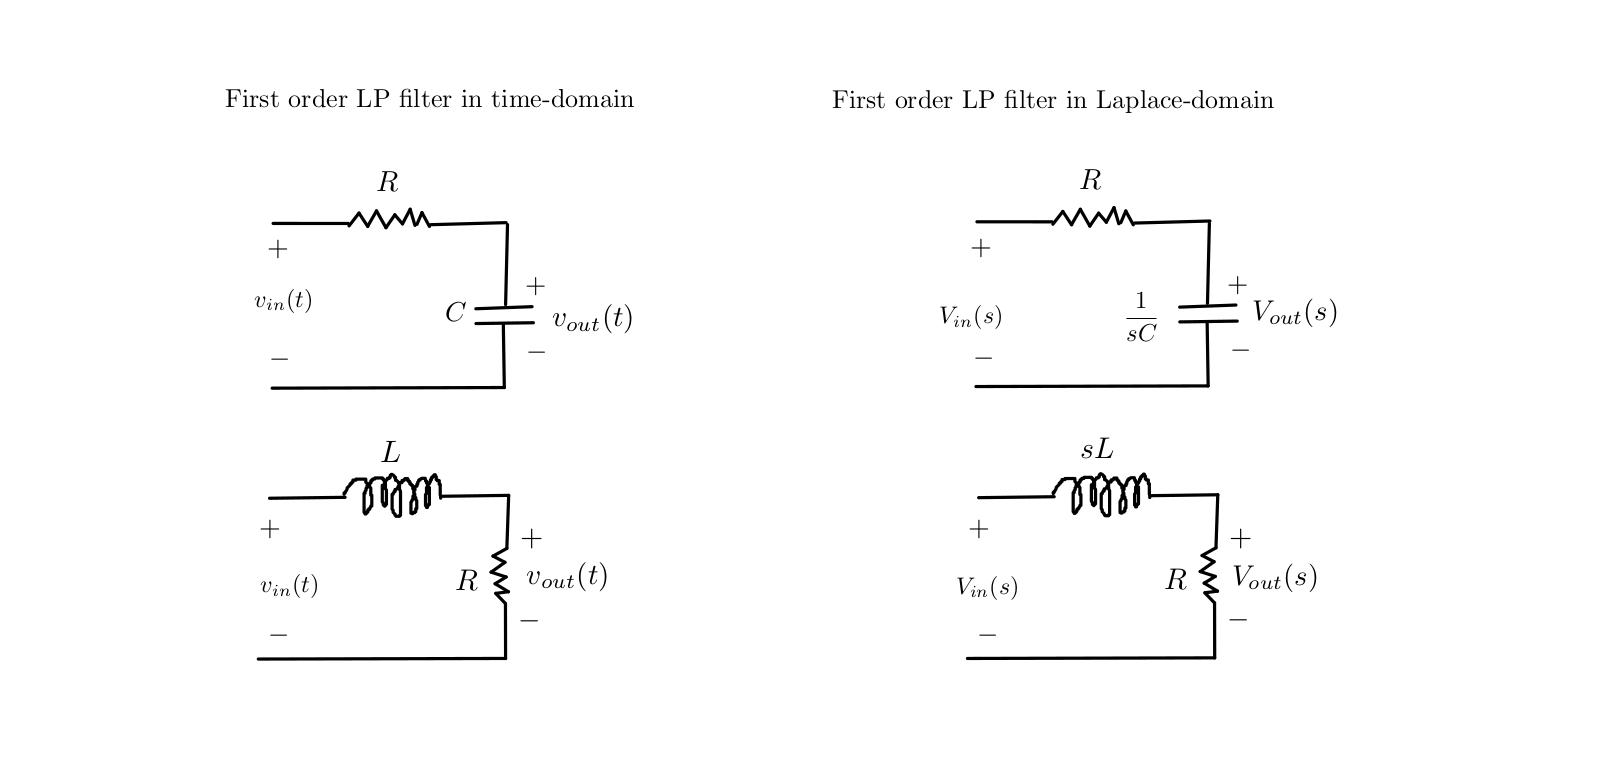
\includegraphics[width=1\textwidth]{2.jpg}
			\caption{First order LP filter in time and Laplace domain}			\label{fig:re2}
		\end{figure}

\end{frame}
\begin{frame}{Thiết kế bộ lọc tương tự}
Ta tìm hàm truyền của hai cấu trúc bộ lọc trên:
$$H(s)=\frac{\frac{1}{sC}}{R+\frac{1}{sC}}=\frac{1}{sRC+1}$$
$$H(s)=\frac{R}{R+sL}=\frac{1}{s\frac{L}{R}+1}$$
Ta đặt $\tau=RC$ hoặc $\tau=\frac{L}{R}$ là hằng số thời gian (time constant), ta thấy cả hai hàm truyền đều có chung dạng công thức: $$H(s)=\frac{1}{s\tau+1}$$
Ta muốn tìm đáp ứng tần số của hệ thống (bộ lọc là hệ thống nhân quả ổn định), thay $s=j\Omega$, ta có:
$$H(j\Omega)=\frac{1}{j\Omega\tau+1}\Rightarrow |H(j\Omega)|=\frac{1}{\sqrt{1+(\Omega\tau)^2}}$$
Hiển nhiên: $$H(j\Omega)=\frac{1}{j\Omega\tau+1}=\frac{1-j\Omega\tau}{1+(\Omega\tau)^2}\Rightarrow \angle H(j\Omega)=-\arctan{(\Omega\tau)}$$
Ta muốn biểu diễn đáp ứng tần số và đáp ứng pha của bộ lọc bằng \textbf{thang tuyến tính} và \textbf{thang dB}.
\end{frame}
\begin{frame}{Thiết kế bộ lọc tương tự}
\begin{figure}[h]
			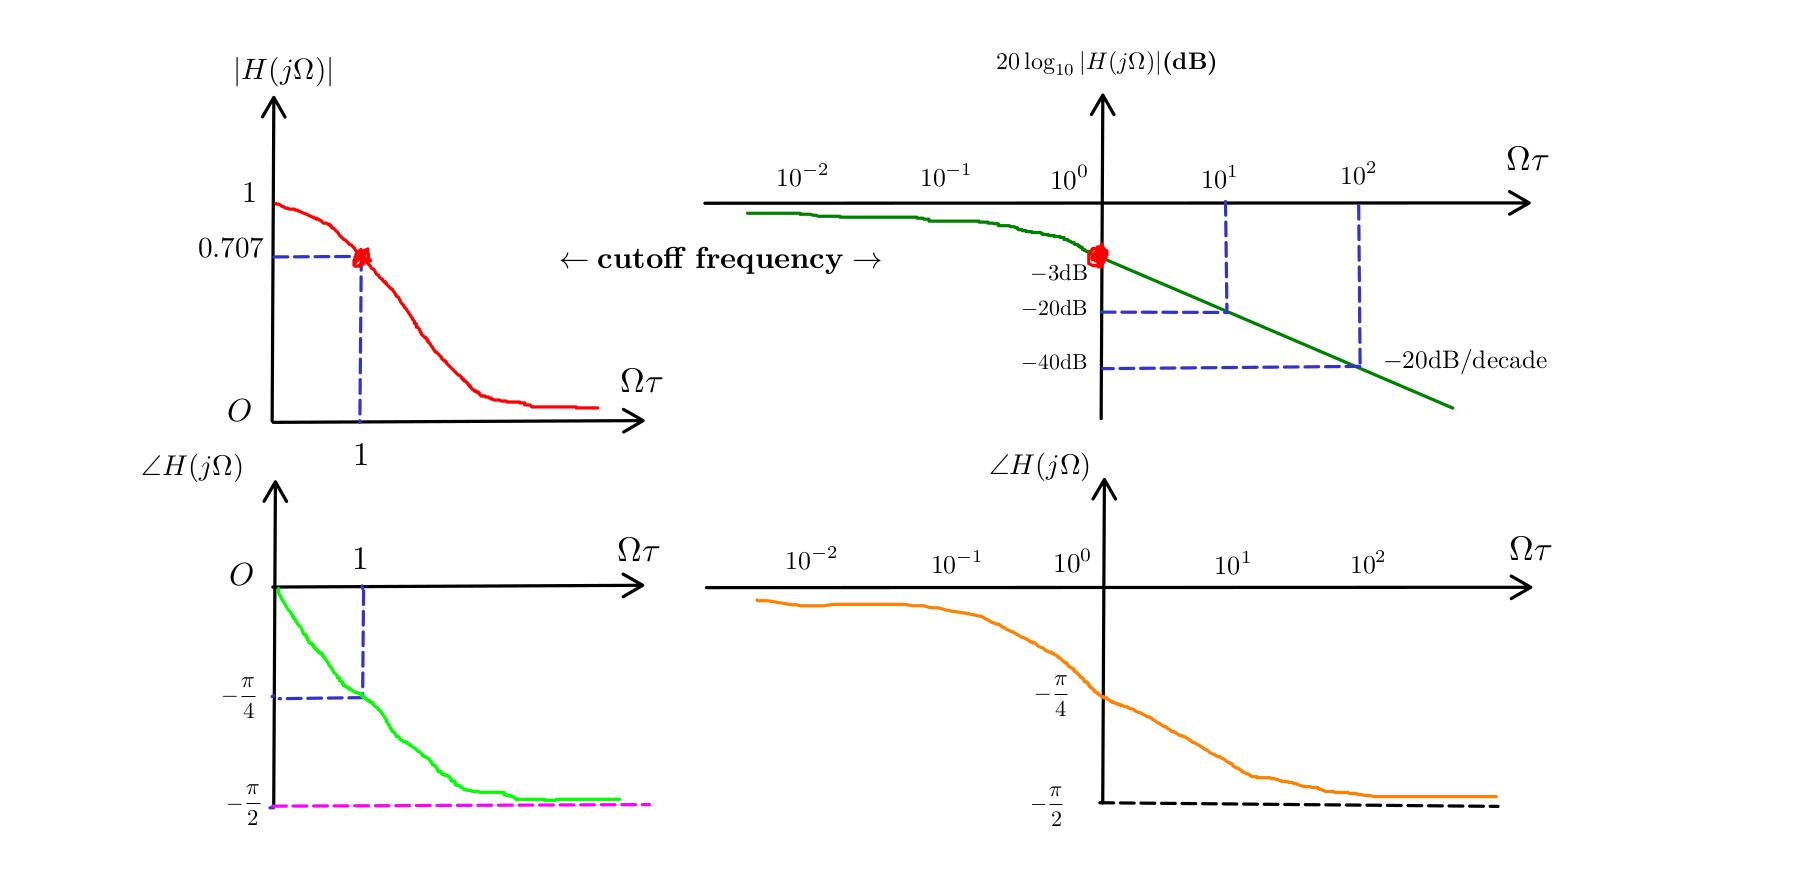
\includegraphics[width=1.1\textwidth]{3.jpg}
			\caption{First order LP filter in linear and dB scale}			\label{fig:re2}
		\end{figure}

\end{frame}
\begin{frame}{Thiết kế bộ lọc tương tự}
	Ta thấy rằng bộ lọc thông thấp (từ giờ ta sẽ gọi tắt các bộ lọc theo thuật ngữ tiếng Anh) LP có độ lợi $G=-20$dB/decade (gain), và tín hiệu sau khi đi qua bộ lọc có hiện tượng \textbf{méo pha} được thể hiện rất rõ trên phổ. Đối với bộ lọc tương tự đơn giản, ta \alert{không thể khắc phục được hiện tượng méo pha}, ta chỉ có thể cải thiện giá trị \textbf{độ lợi G} mà thôi.

	\\Đối với bộ lọc tương tự đơn giản, ta định nghĩa khái niệm hằng số \textbf{tần số cắt} (cutoff frequency) chính là \alert{tần số biên}, tại giá trị này \textbf{năng lượng} của tín hiệu gốc bị \textbf{suy hao một nửa}. 
	\\ Nếu ta quy đổi theo thang dB, độ lợi $G_{c}$ tại tần số cắt là:
	$$G_{c}=20\log_{10}\left(\frac{1}{\sqrt{1+1}}\right)=-3\text{dB}$$
	Từ đáp ứng biên độ của bộ lọc LP bậc 1: $$|H(j\Omega)|=\frac{1}{\sqrt{1+(\Omega\tau)^2}}$$
	 Để giảm độ lợi $G$ xuống càng thấp càng tốt, ta thiết kế bộ lọc LP có bậc $n$ tổng quát có phương trình đáp ứng biên độ như sau:
	 $$|H(j\Omega)|=\frac{1}{\sqrt{1+(\Omega\tau)^{\alert{2n}}}}$$
	 Ta giới thiệu một vài sơ đồ mạch bộ lọc tương tự LP có bậc $n=2$ và dạng tổng quát (Cauer form). \textbf{Lưu ý: bậc bộ lọc bằng số phần tử dự trữ năng lượng trong mạch}.
\end{frame}
\begin{frame}{Thiết kế bộ lọc tương tự}
\begin{figure}[h]
			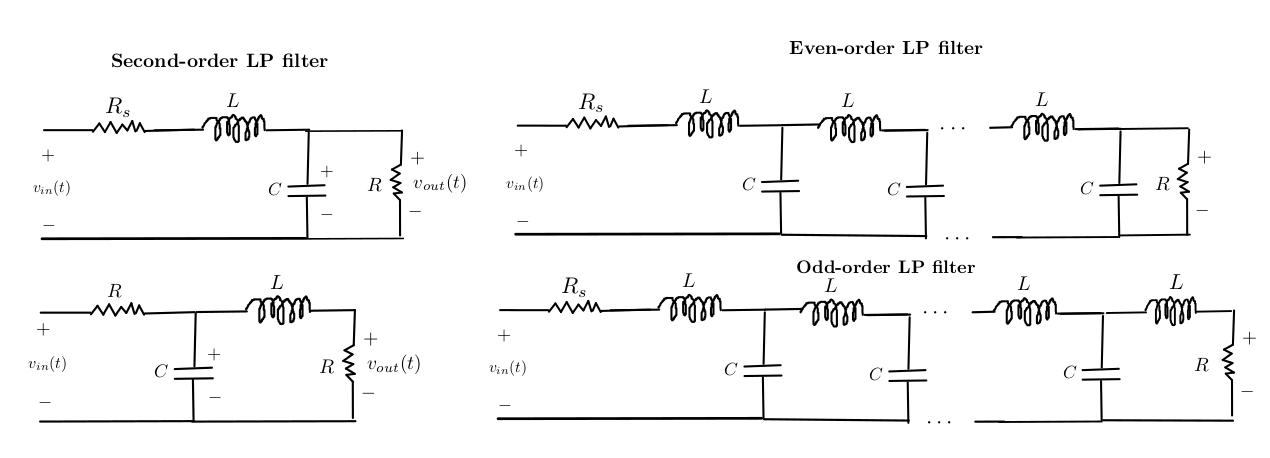
\includegraphics[width=1.1\textwidth]{4.jpg}
			\caption{Second order LP filter and higher order in Cauer form}			\label{fig:re2}
		\end{figure}

\end{frame}
\begin{frame}{Thiết kế bộ lọc tương tự}
\begin{figure}[h]
			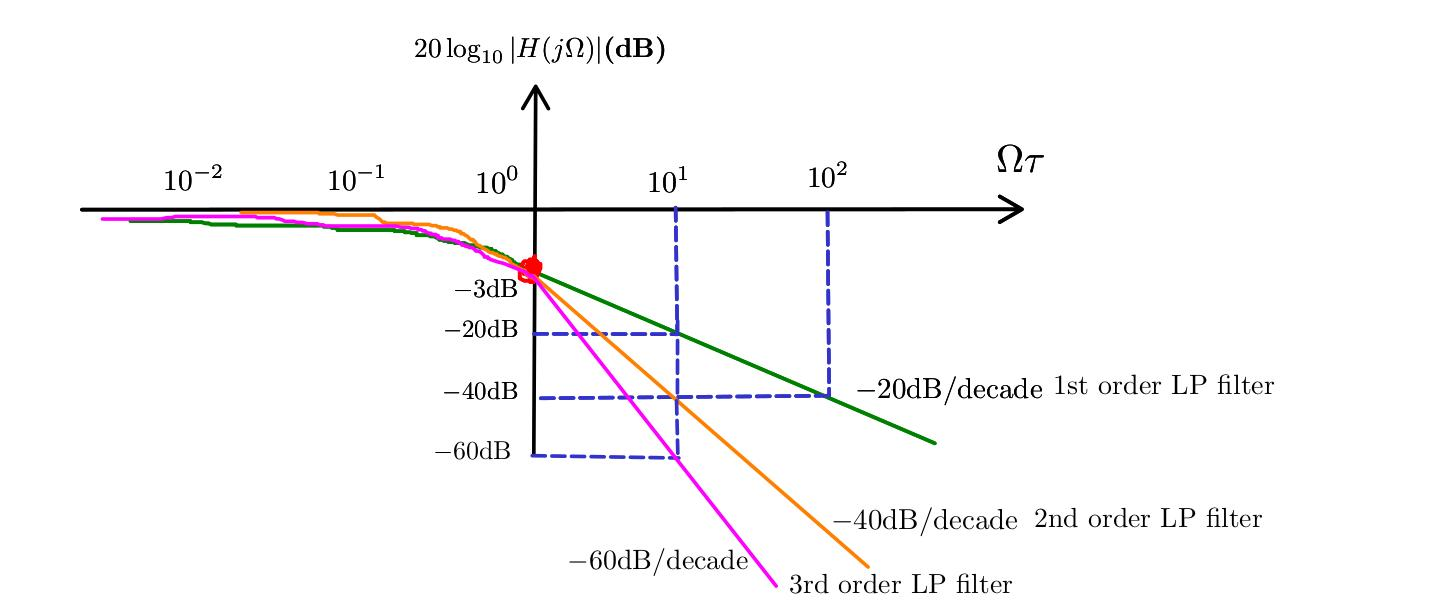
\includegraphics[width=1.1\textwidth]{5.jpg}
			\caption{Frequency response in dB scale of high order LP filter}			\label{fig:re2}
		\end{figure}

\end{frame}
\begin{frame}{Thiết kế bộ lọc tương tự}
\begin{itemize}
	\item[-] Bộ lọc thông cao (HP)
\end{itemize}
\subsubsection{Bộ lọc thông cao (HP)}
Cũng tương tự như bộ lọc LP, ta bắt đầu từ việc khảo sát bộ lọc HP bậc 1 đơn giản nhất có sơ đồ mạch như sau:
\begin{figure}[h]
			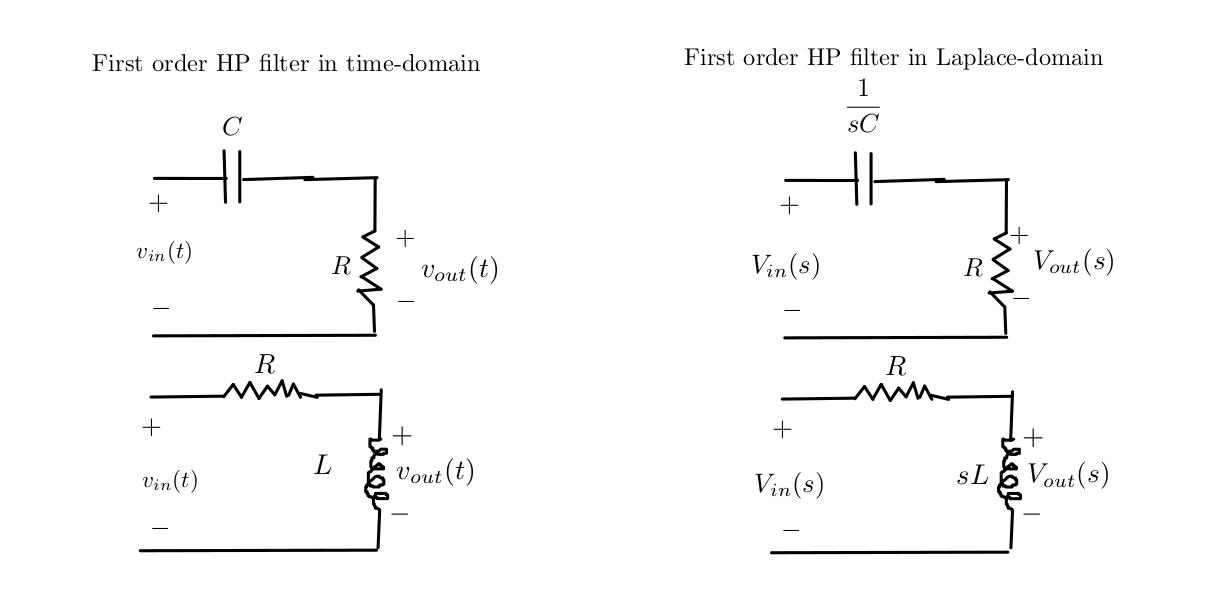
\includegraphics[width=1.1\textwidth]{6.jpg}
			\caption{First order HP filter in time and Laplace domain}			\label{fig:re2}
		\end{figure}

\end{frame}
\begin{frame}{Thiết kế bộ lọc tương tự}
Ta cũng xây dựng được biểu thức hàm truyền của hai bộ lọc HP trên như sau:
$$H(s)=\frac{R}{R+\frac{1}{sC}}=\frac{sRC}{sRC+1}$$
$$H(s)=\frac{sL}{sL+R}=\frac{s\frac{L}{R}}{s\frac{L}{R}+1}$$
Đặt $\tau=RC$ hay $\tau=\frac{L}{R}$ là hằng số thời gian (time constant), ta thu được dạng hàm truyền của bộ lọc HP: $$H(s)=\frac{s\tau}{s\tau+1}$$
Hiển nhiên đây là hệ thống nhân quả ổn định, ta thay $s=j\Omega$ để tìm đáp ứng tần số của bộ lọc HP: $$H(j\Omega)=\frac{j\Omega\tau}{j\Omega\tau+1}\Rightarrow |H(j\Omega)|=\frac{\Omega\tau}{\sqrt{(\Omega\tau)^2+1}}=\frac{1}{\sqrt{1+\left(\frac{1}{\Omega\tau}\right)^2}}$$
Dễ thấy: $$H(j\Omega)=\frac{j\Omega\tau(1-j\Omega\tau)}{1+(\Omega\tau)^2}=\frac{(\Omega\tau)^2+j\Omega\tau}{1+(\Omega\tau)^2}\Rightarrow\angel \angle H(j\Omega)=\arctan{\frac{1}{\Omega\tau}}$$
Tương tự, ta cũng vẽ đồ thị đáp ứng biên độ và pha của bộ lọc HP bằng thang tuyến tính và thang dB.
\end{frame}
\begin{frame}{Thiết kế bộ lọc tương tự}
\begin{figure}[h]
			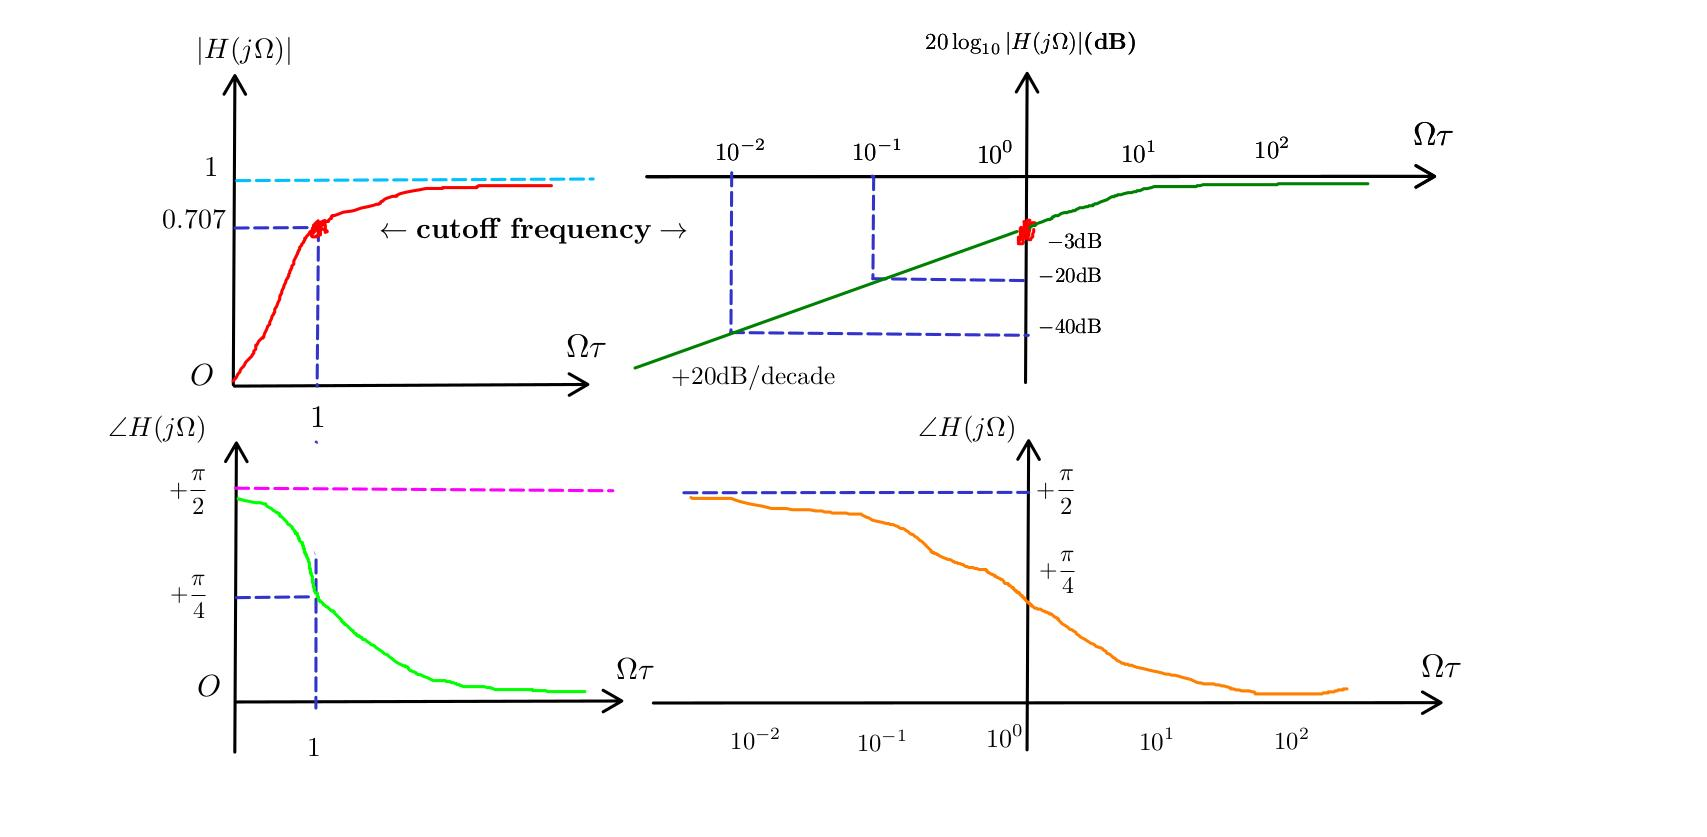
\includegraphics[width=1.1\textwidth]{7.jpg}
			\caption{First order HP filter in linear and dB scale}			\label{fig:re2}
		\end{figure}

\end{frame}
\begin{frame}{Thiết kế bộ lọc tương tự}
Tương tự với bộ lọc LP, tần số cắt cũng nằm tại vị trí $-3$dB. Từ phương trình đáp ứng biên độ của bộ lọc HP bậc 1:  $$|H(j\Omega)|=\frac{1}{\sqrt{1+\left(\frac{1}{\Omega\tau}\right)^{2}}}$$
Ta cũng có phương trình đáp ứng biên độ của bộ lọc HP bậc $n$ tổng quát:
$$|H(j\Omega)|=\frac{1}{\sqrt{1+\left(\frac{1}{\Omega\tau}\right)^{2n}}}$$
Dễ thấy bộ lọc HP \alert{chính là phiên bản "đảo ngược"} của bộ lọc LP. Đây là nhận định cực kì quan trọng đóng vai trò cơ sở cho thuật toán thiết kế bộ lọc HP được nghiên cứu sau này.
\\ Ta giới thiệu một vài sơ đồ mạch tương tự cấu trúc bộ lọc HP bậc 2 và cao hơn như dưới đây. \textbf{Lưu ý: cũng giống như bộ lọc LP, bậc bộ lọc bằng số phần tử dự trữ năng lượng trong mạch.}
\end{frame}
\begin{frame}{Thiết kế bộ lọc tương tự}
\begin{figure}[h]
			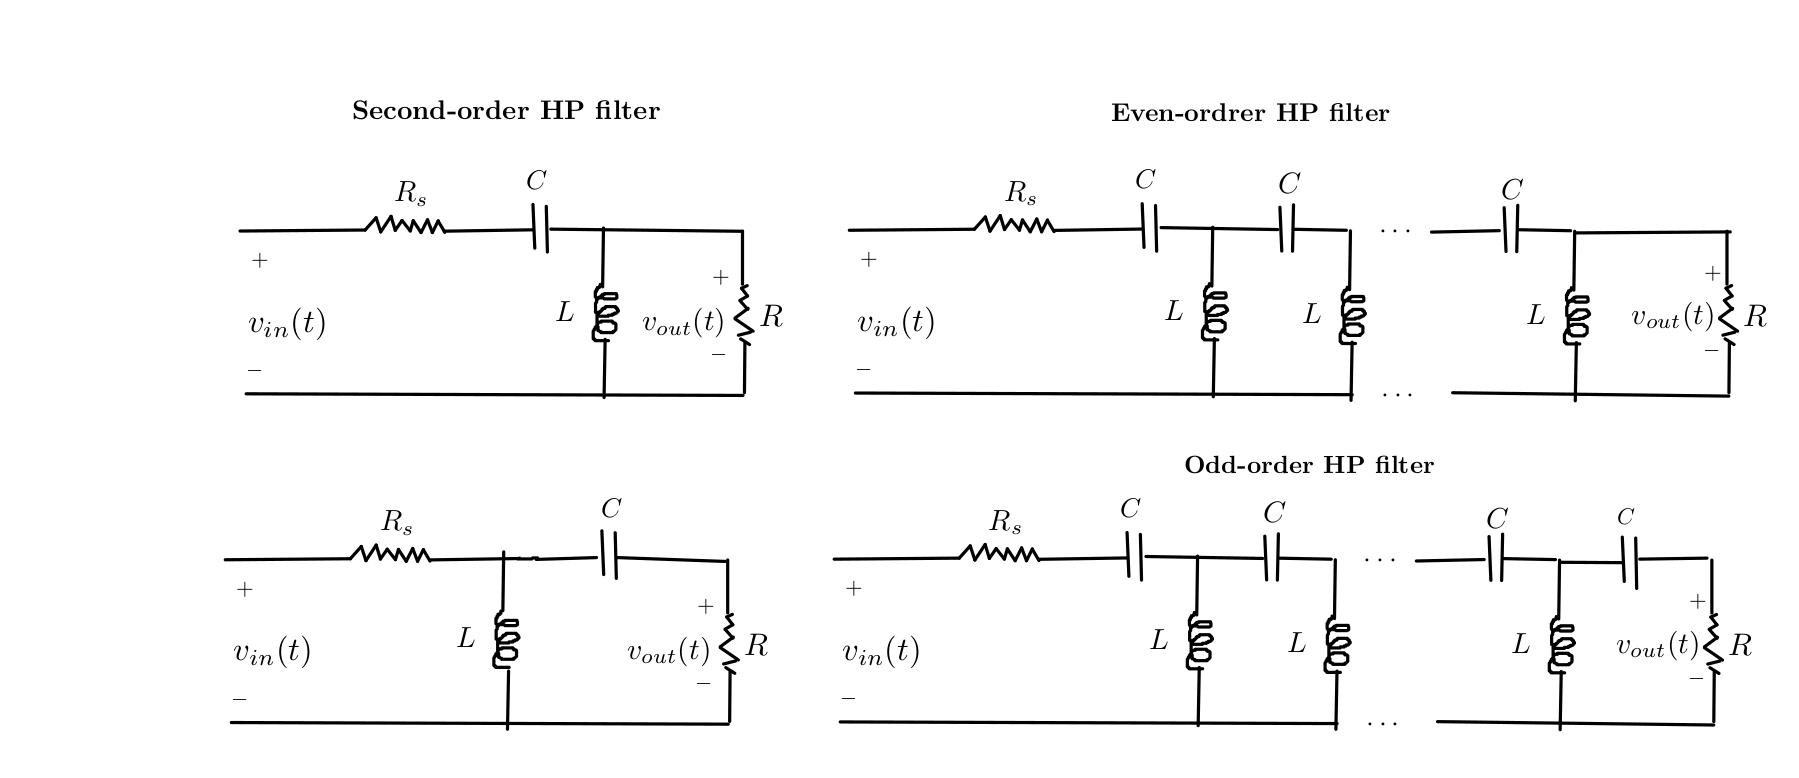
\includegraphics[width=1.1\textwidth]{8.jpg}
			\caption{Second order HP filter and higher in Cauer form}			\label{fig:re2}
		\end{figure}


\end{frame}
\begin{frame}{Thiết kế bộ lọc tương tự}
\begin{figure}[h]
			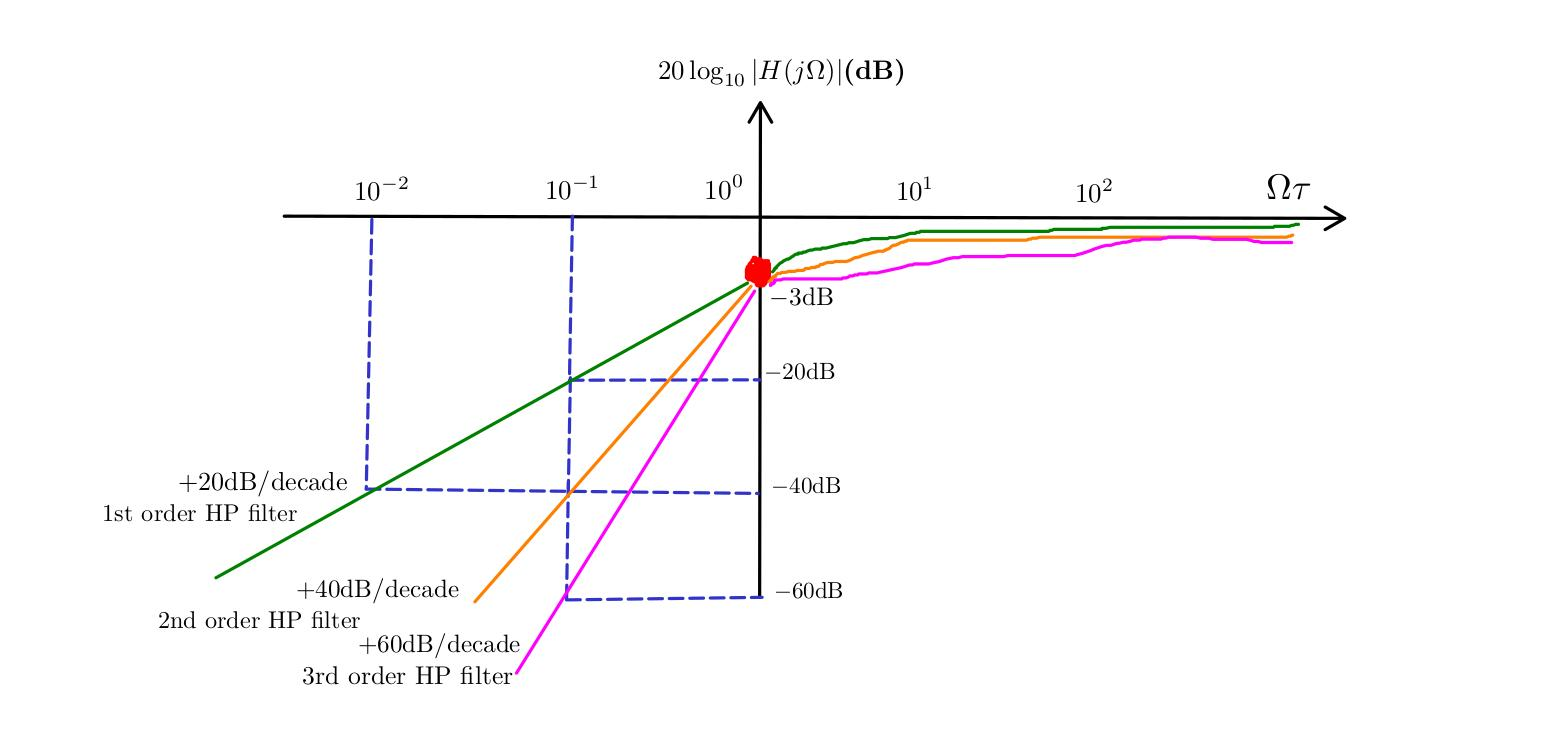
\includegraphics[width=1.1\textwidth]{9.jpg}
		\caption{Frequency response in dB scale of high order HP filter}			\label{fig:re2}
		\end{figure}

\end{frame}
\begin{frame}{Thiết kế bộ lọc tương tự}
\subsubsection{Bộ lọc thông dải (BP)}
\begin{itemize}
	\item[-] Bộ lọc thông dải (BP)
\end{itemize}

\begin{figure}[h]
			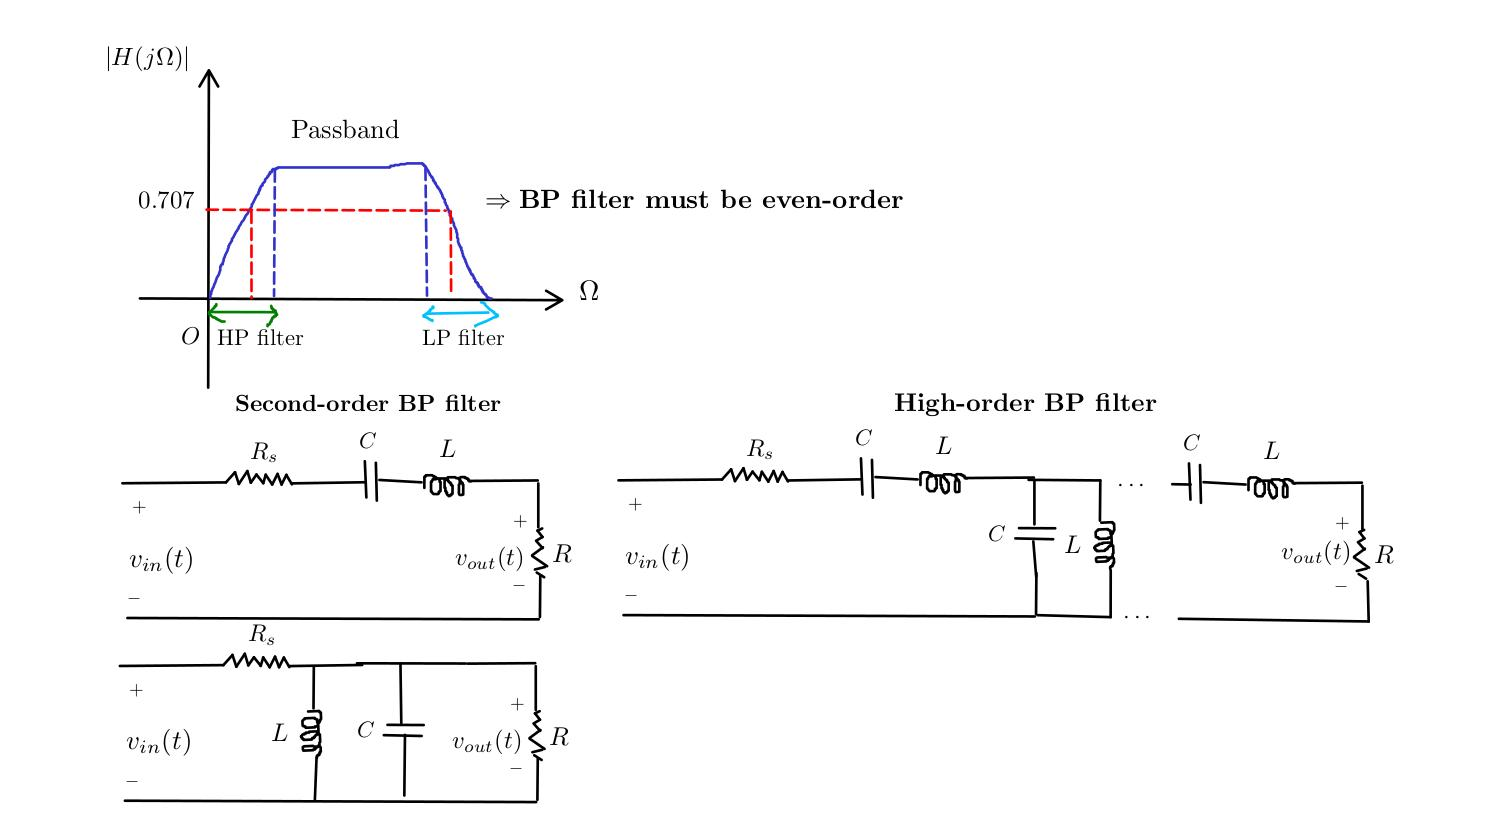
\includegraphics[width=1.1\textwidth]{10.jpg}
		\caption{Bandpass filter}			\label{fig:re2}
		\end{figure}
\end{frame}
\begin{frame}{Thiểt kế bộ lọc tương tự}
\begin{itemize}
	\item[-] Bộ lọc chặn dải (BS)
\end{itemize}
\subsubsection{Bộ lọc chặn dải (BS)}
\begin{figure}[h]
			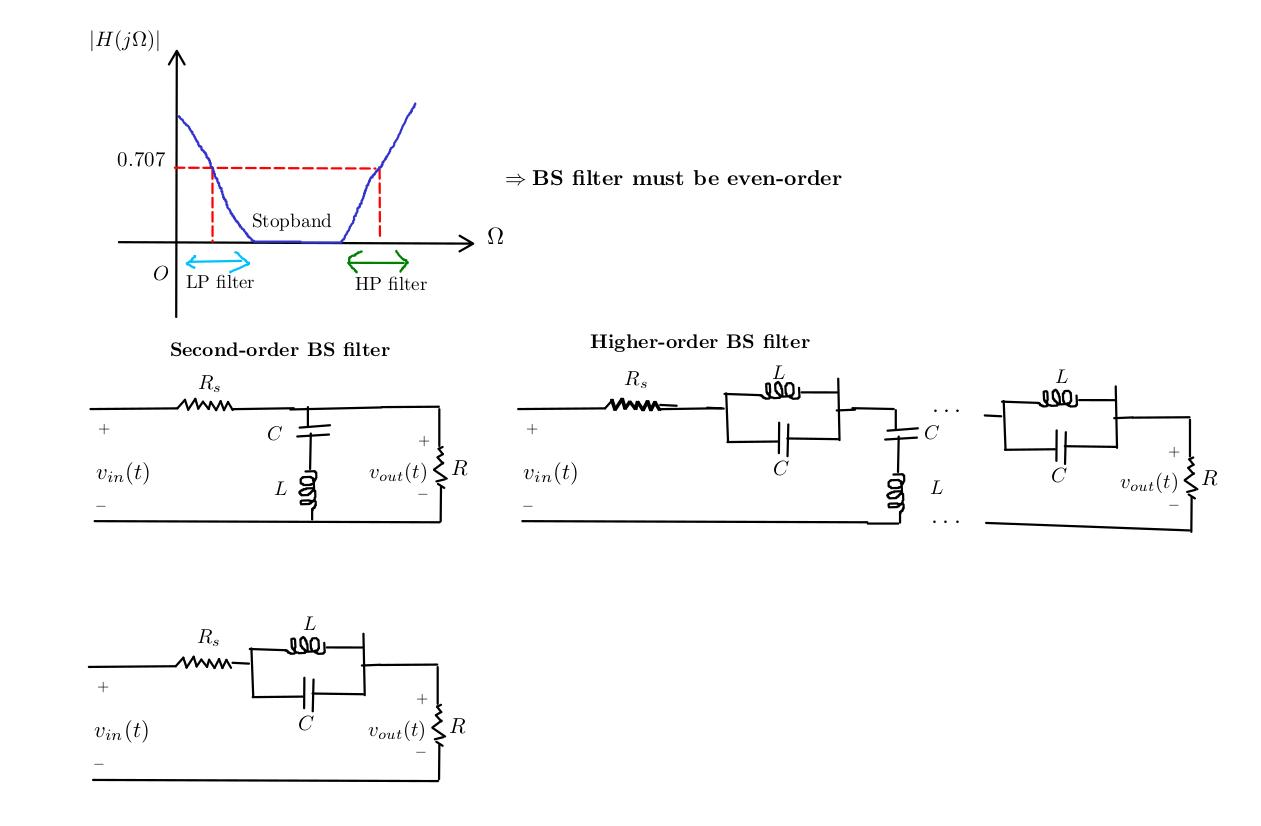
\includegraphics[width=1\textwidth]{11.jpg}
		\caption{Bandstop filter}			\label{fig:re2}
		\end{figure}

\end{frame}
\begin{frame}{Thiết kế bộ lọc tương tự}
\subsection{Thiết kế bộ lọc LP}
\subsubsection{Bộ lọc Butterworth}
\begin{itemize}
	\item Thiết kế bộ lọc LP
\end{itemize}

Bộ lọc LP là loại bộ lọc \textbf{dễ thiết kế nhất} và là \alert{bộ lọc cơ sở để thiết kế các loại bộ lọc khác}. Ta giới thiệu 2 họ bộ lọc tương tự LP cơ bản nhất trong giới hạn chương trình học phần, đó là \textbf{bộ lọc Butterworth} và \textbf{bộ lọc Chebyshev}.
\begin{itemize}
	\item[-] Bộ lọc Butterworth
\end{itemize}
Bộ lọc LP Butterworth là loại bộ lọc đơn giản nhất có đáp ứng biên độ tổng quát:
$$|H(j\Omega)|=\frac{1}{\sqrt{1+\left(\frac{\Omega}{\Omega_{c}}\right)^{2n}}}\Rightarrow |H^{2}(j\Omega)|=\frac{1}{1+\left(\frac{\Omega}{\Omega_{c}}\right)^{2n}}$$
với $\Omega_{c}$ là \alert{tần số cắt của bộ lọc} tại độ lợi \alert{$G_{c}=-3$dB}, và $n$ là \textbf{bậc của bộ lọc}.
\\ Ta rất dễ nhận ra rằng, phương trình đáp ứng biên độ của họ bộ lọc LP Butterworth \textbf{giống} với dạng đáp ứng biên độ bộ lọc LP được thiết kế bằng các linh kiện điện tử thụ động đơn giản $R,L,C$ đã phân tích ở trên.
\\ Hay nói cách khác, phương trình đáp ứng biên độ của bộ lọc LP Butterworth \textbf{lấy ý tưởng từ phương pháp thiết kế bộ lọc LP thụ động đơn giản}.
\\ Ta biểu diễn đáp ứng biên độ của bộ lọc LP như sau:
\end{frame}
\begin{frame}{Thiết kế bộ lọc tương tự}
\begin{figure}[h]
			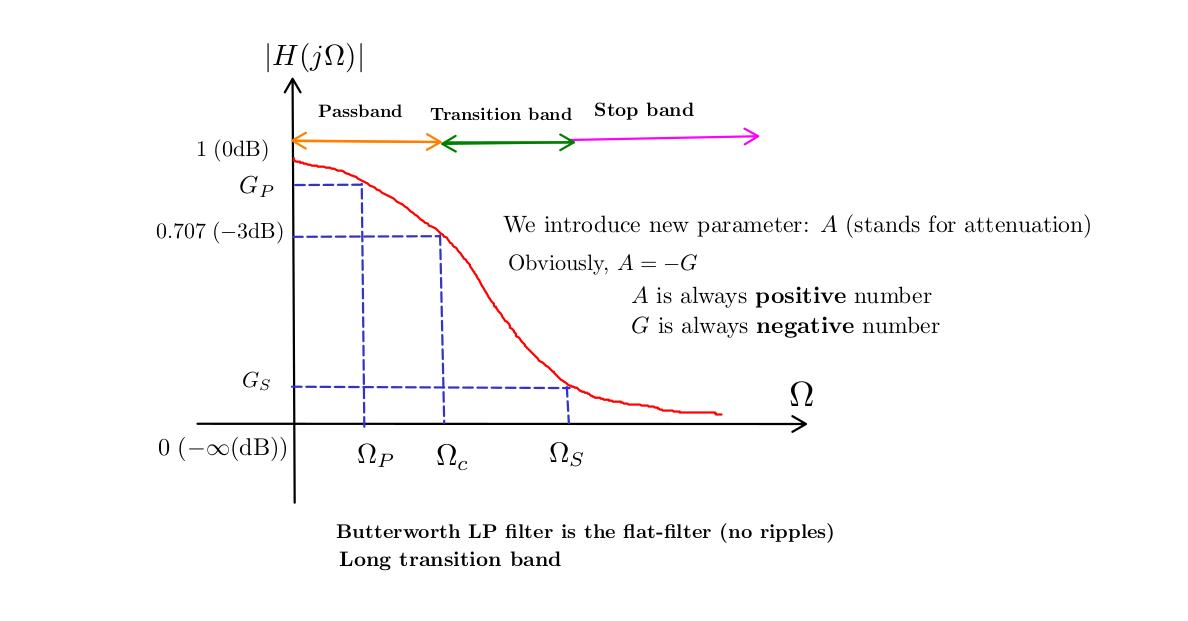
\includegraphics[width=1\textwidth]{12.jpg}
		\caption{Frequency response of Butterworth LP filter}			\label{fig:re2}
		\end{figure}

\end{frame}
\begin{frame}{Thiết kế bộ lọc tương tự}
	Bản chất của bài toán thiết kế bộ lọc là tìm \alert{hàm truyền $H(s)$} của hệ thống từ công thức đáp ứng tần số $|H(j\Omega)|$. Sau đó từ hàm truyền tìm được, người ta sẽ sử dụng các linh kiện điện tử phù hợp như $R,L,C$ hay Op-Amp để lắp ráp bộ lọc tương ứng.
\\ Để dễ dàng hình dung hơn về quy trình thiết kế bộ lọc, ta sẽ xét 3 ví dụ cơ bản sau:
\begin{enumerate}
	\item[1] Thiết kế bộ lọc Butterworth LP bậc 1 có tần số cắt $\alert{\Omega_{C}=1\;\text{(rad/s)}}$.
Từ phương trình đáp ứng tần số (thực ra đáp ứng biên độ là tên gọi chính xác hơn về thuật ngữ), ta có:
$$|H(j\Omega)|=\frac{1}{\sqrt{1+\Omega^2}}\Rightarrow |H^2(j\Omega)|=\frac{1}{1+\Omega^2}$$
Do bộ lọc là hệ thống ổn định, nên ta luôn có $\alert{s=j\Omega}$. Từ công thức tích liên hợp phức cơ bản, ta có kết quả rất quan trọng: $$\alert{|H^2(j\Omega)|=H(j\Omega)H(j\Omega)^*=H(j\Omega)H(-j\Omega)=H(s)H(-s)}$$
Thay toàn bộ $s$ vào phương trình đáp ứng tần số, ta thu được:
$$|H^2(j\Omega)|=\frac{1}{1+\Omega^2}\Rightarrow H(s)H(-s)=\frac{1}{1+\left(\frac{s}{j}\right)^2}=\frac{1}{-s^2+1}$$
Giải phương trình điểm cực của $H(s)H(-s)$, ta thu được $2$ điểm cực $s=\pm 1$, thế nhưng ta muốn tìm \alert{hàm truyền $H(s)$} có nghiệm cực sao cho đảm bảo \textbf{hệ thống ổn định}, tương đương với $\Re{(s)}<0$. Vậy ta chọn nghiệm cực $s=-1$ và thu được hàm truyền: $$H(s)=\frac{1}{s+1}$$
	\end{enumerate}

\end{frame}
\begin{frame}{Thiết kế bộ lọc tương tự}
	\begin{enumerate}
		\item[2] Thiết kế bộ lọc Butterworth LP bậc 2 có tần số cắt $\alert{\Omega_{C}=1\;\text{(rad/s)}}$.  Thực hiện với quy trình tương tự, ta cũng có:

$$|H(j\Omega)|=\frac{1}{\sqrt{1+\Omega^4}}\Rightarrow |H^2(j\Omega)|=\frac{1}{1+\Omega^4}$$
Thay $s=j\Omega$, ta cũng có:

$$|H^2(j\Omega)|=\frac{1}{1+\Omega^4}\Rightarrow H(s)H(-s)=\frac{1}{1+\left(\frac{s}{j}\right)^4}=\frac{1}{s^4+1}$$
Từ phương trình nghiệm cực $s^4+1=0$, ta cần phải giải ra $2$ nghiệm phức thỏa mãn $\Re{(s)}<0$:
$$s^4+1=0\Rightarrow(s^2-j)(s^2+j)=0$$
\begin{equation*}
\begin{cases}
	s^2=j=\alert{e^{j\frac{\pi}{2}}}\\
	s^2=-j=\alert{e^{-j\frac{\pi}{2}}}\\
\end{cases}
\Rightarrow
\begin{cases}
	s=e^{j\frac{\pi}{4}}\\
	s=-e^{j\frac{\pi}{4}}\\

	s=e^{-j\frac{\pi}{4}}\\
	s=-e^{-j\frac{\pi}{4}}\\
\end{cases}
\end{equation*}
Chọn cặp nghiệm $s=-e^{\pm j\frac{\pi}{4}}=-0.707\pm j0.707$, dùng định lý Viete đảo, ta tìm được: $$H(s)=\frac{1}{s^2+\sqrt{2}s+1}$$
	\end{enumerate}
\end{frame}
\begin{frame}{Thiết kế bộ lọc tương tự}

	\begin{enumerate}
		\item[3] Thiết kế bộ lọc Butterworth LP bậc 3 có tần số cắt $\alert{\Omega_{C}=1\;\text{(rad/s)}}$.  Thực hiện với quy trình tương tự, ta cũng có:

$$|H(j\Omega)|=\frac{1}{\sqrt{1+\Omega^6}}\Rightarrow |H^2(j\Omega)|=\frac{1}{1+\Omega^6}$$
Thay $s=j\Omega$, ta cũng có:

$$|H^2(j\Omega)|=\frac{1}{1+\Omega^6}\Rightarrow H(s)H(-s)=\frac{1}{1+\left(\frac{s}{j}\right)^6}=\frac{1}{-s^6+1}$$
Từ phương trình nghiệm cực $-s^6+1=0$, ta cần phải giải ra $3$ nghiệm phức thỏa mãn $\Re{(s)}<0$:
$$-s^6+1=0\Rightarrow(s^2-1)(s^4+s^2+1)=0$$

\begin{equation*}
\begin{cases}
s=\pm 1\\
s^2=e^{\pm j\frac{2\pi}{3}}\\
\end{cases}
\Rightarrow
\begin{cases}
	s=\pm 1\\
	s=\pm e^{j\frac{\pi}{3}}\\
	s=\pm e^{-j\frac{\pi}{3}}\\
\end{cases}
\end{equation*}
Ta chọn 3 nghiệm $s=-1$, $s=-e^{\pm j\frac{\pi}{3}}$, dùng định lý Viete đảo, ta tìm được:
$$H(s)=\frac{1}{(s+1)(s^2+s+1)}$$
\end{enumerate}
\end{frame}
\begin{frame}{Thiết kế bộ lọc tương tự}
Tổng quát, bài toán thiết kế bộ lọc LP Butterworth bậc $n$ có $\Omega_{C}=1\;$(rad/s) tương đương với tìm đa thức có nghiệm \textbf{là nghiệm phần thực âm} của phương trình điểm cực:
$$\left(\frac{s}{j}\right)^{2n}=-1=e^{j\pi(2k-1)}\Rightarrow s^{2n}=e^{j\pi(2k-1)}e^{j\pi n}=e^{j\pi(n+2k-1)}$$
Vậy ta tìm được các nghiệm: $$s_{k}=e^{\frac{j\pi(n+2k-1)}{2n}}\;(k=1,2,\cdots,2n)$$
Chọn các nghiệm thỏa mãn $\Re{(s_{k})}<0$, ta thu được đa thức cực tương ứng của bộ lọc: $$\prod_{\Re{(s_{k})}<0}(s-s_{k})$$
Ta gọi đa thức cực trên là \textbf{đa thức Butterworth} có bậc $N$, được kí hiệu là $B_{N}(s)$.
\\ Các nhà toán học đã tìm được bảng \textbf{đa thức Butterworth} như sau:
\end{frame}
\begin{frame}{Thiết kế bộ lọc tương tự}
\begin{figure}[h]
			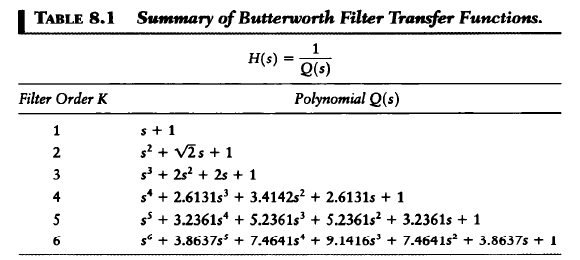
\includegraphics[width=0.7\textwidth]{phpe46ibx.png}
		\caption{Butterworth polynomials table}			\label{fig:re2}
		\end{figure}
Đương nhiên, bằng cách tính tay như đã trình bày ở 3 ví dụ trước, ta đều có thể tự nghiệm thu lại các đa thức Butterworth trong bảng trên. Thế nhưng, để cho tiện ta sẽ dùng thẳng bảng đa thức này luôn (đi thi bảng cũng được in vào đề).
\\ Ta thu được một kết quả quan trọng:  \\\textbf{\alert{Bộ lọc Butterworth LP bậc $N$ có tần số cắt chuẩn hóa (normalized frequency) $\Omega_{C}=1$ (rad/s) có hàm truyền:}} $$\alert{H(s)=\frac{1}{B_{N}(s)}}$$
\end{frame}
\begin{frame}{Thiết kế bộ lọc tương tự}
Ta mở rộng kết quả trên để tìm hàm truyền của bộ lọc Butterworth LP có \alert{tần số cắt $\Omega_{C}$ không chuẩn hóa}, dễ thấy từ đồ thị đáp ứng biên độ của hai bộ lọc:
\begin{figure}[h]
	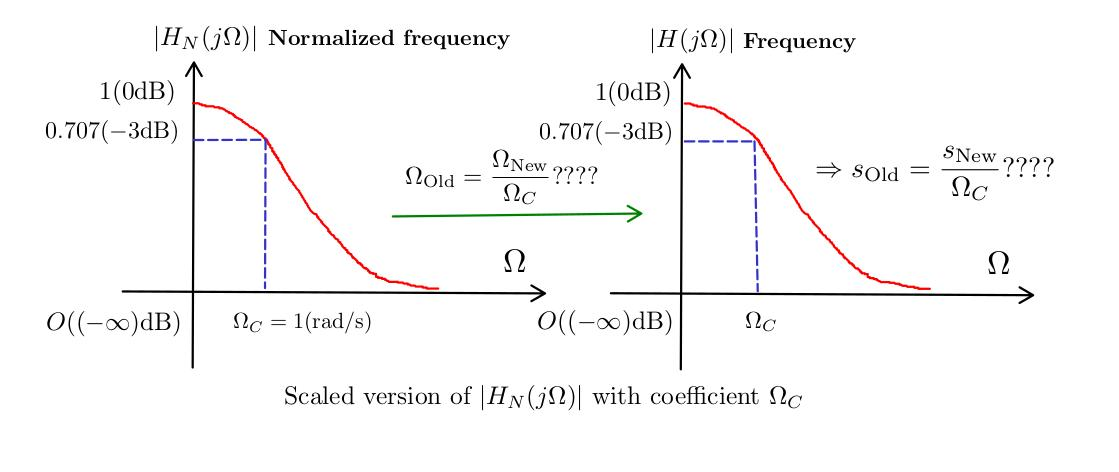
\includegraphics[width=0.9\textwidth]{13.jpg}
	\caption{Design Butterworth LP filter}			\label{fig:re2}
		\end{figure}
		Ta dễ dàng nhận thấy rằng ta phải \textbf{định nghĩa thêm các kí hiệu mới tương ứng với các loại bộ lọc} để tránh nhầm lẫn và rối. Hay nói cách khác, các kí hiệu phải được \alert{hệ thống} một cách thuận tiện và chính xác.

\end{frame}
\begin{frame}{Thiết kế bộ lọc tương tự}
Đối với bộ lọc Butterworth LP có \alert{tần số cắt chuẩn hóa $\Omega_{C}=1$ (rad/s)}, ta kí hiệu:
\begin{enumerate}
	\item[1] Kí hiệu tần số góc: $\lambda$
	\item[2] Kí hiệu biến Laplace: $p$
	\item[3] Kí hiệu hàm truyền: $H_{N}(p)$
\end{enumerate}

Đối với bộ lọc Butterworth LP có \alert{tần số cắt không chuẩn hóa} (hay gọi là tần số cắt thường), ta kí hiệu:
\begin{enumerate}
	\item[1] Kí hiệu tần số góc: $\Omega$
	\item[2] Kí hiệu biến Laplace: $s$
	\item[3] Kí hiệu hàm truyền: $H(s)$
\end{enumerate}
Hệ thống kí hiệu này sẽ theo ta cho đến hết môn học, nên ta cần phải nắm rất chắc và không được nhầm lẫn ý nghĩa của chúng với nhau. Mình sẽ liên tục nhắc lại hệ thống kí hiệu này ở từng mục nhỏ.
\\Sử dụng hệ thống kí hiệu trên, ta thu được: 
$$\lambda=\frac{\Omega}{\Omega_{C}}\Rightarrow p=\frac{s}{\Omega_{C}}\Rightarrow H(s)=H_{N}\left(\frac{s}{\Omega_{C}}\right)$$
$$H_{N}(p)=\frac{1}{B_{N}(p)}$$
\end{frame}
\begin{frame}{Thiết kế bộ lọc tương tự}
	Ví dụ: thiết kế bộ lọc Butterworth LP bậc 1 có tần số cắt $\Omega_{C}=4$ (rad/s).	\\ Từ bảng đa thức Butterworth, ta có: $$H_{N}(p)=\frac{1}{p+1}$$ Thay: $$p=\frac{s}{\Omega_{C}}$$ Ta thu được: $$H(s)=\frac{1}{\frac{s}{4}+1}=\frac{4}{s+4}$$
Hai thông số quan trọng nhất trong thiết kế là \textbf{bậc $N$} và \textbf{tần số cắt $\Omega_{C}$} của bộ lọc.
\\ Ta tuần tự "tổng quát hóa" bài toán thiết kế bộ lọc Butterworth LP như sau:
\\ \textbf{Biết bậc $N$ và $\Omega_{C}=1$ (rad/s)} $\rightarrow$ \textbf{Biết bậc $N$ và $\Omega_{C}$} $\rightarrow$ \textbf{Biết 4 thông số cơ bản của bộ lọc}
\end{frame}
\begin{frame}{Thiết kế bộ lọc tương tự}
Ví dụ: thiết kế bộ lọc Butterworth LP biết \textbf{4 thông số cơ bản} sau: $\Omega_{P}$, $G_{P}$, $\Omega_{S}$, $G_{S}$. Ta lần lượt biểu diễn các thông số này trên đồ thị đáp ứng tần số:
\begin{figure}[h]
	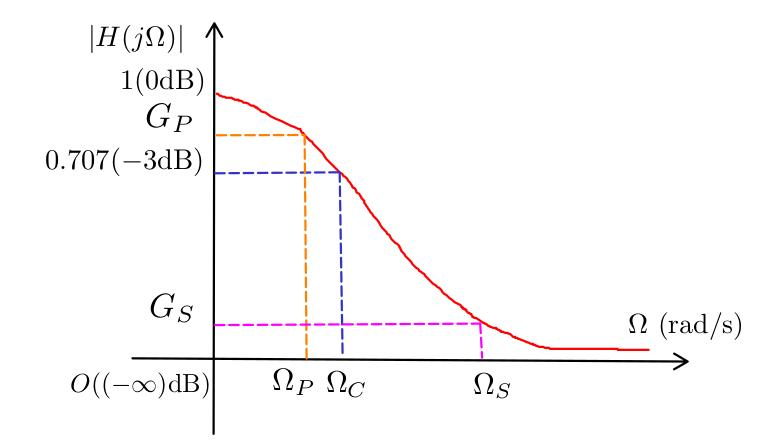
\includegraphics[width=0.9\textwidth]{14.jpg}
	\caption{General Butterworth LP filter frequency response}			\label{fig:re2}
		\end{figure}

\end{frame}
\begin{frame}{Thiết kế bộ lọc tương tự}
 Hiển nhiên ta có:
 \begin{equation*}
\begin{split}
	&G=20\log_{10}|H(j\Omega)|=10\log_{10}|H^2(j\Omega)|=-10\log_{10}\left(1+\left(\frac{\Omega}{\Omega_{C}}\right)^{2n}\right)\\
	&\Rightarrow \left(\frac{\Omega}{\Omega_{C}}\right)^{2n}=10^{\frac{-G}{10}}-1\Rightarrow \alert{\left(\frac{\Omega_{P}}{\Omega_{S}}\right)^{2n}=\frac{10^{\frac{-G_{P}}{10}}-1}{10^{\frac{-G_{S}}{10}}-1}}\\
	&\Rightarrow \alert{n=\log_{10}\left(\frac{10^{\frac{-G_{P}}{10}}-1}{10^{\frac{-G_{S}}{10}}-1}\right)\bigg/2\log_{10}\left(\frac{\Omega_{P}}{\Omega_{S}}\right)}\\
	&\textbf{Lưu ý chọn  $(n=\lceil n\rceil)$}\\
	&\left(\frac{\Omega}{\Omega_{C}}\right)^{2n}=10^{\frac{-G}{10}}-1\Rightarrow \left(\frac{\Omega_{P}}{\Omega_{C}}\right)^{2n}=10^{\frac{-G_{P}}{10}}-1 \Rightarrow \alert{\Omega_{C}=\frac{\Omega_{P}}{\left(10^{\frac{-G_{P}}{10}}-1\right)^{\frac{1}{2n}}}}
\end{split}
\end{equation*}
Nếu đề bài cho $A$, ta chỉ việc đổi dấu $A=-G$:
\begin{equation*}
\begin{split}
	\alert{n=\log_{10}\left(\frac{10^{\frac{A_{P}}{10}}-1}{10^{\frac{A_{S}}{10}}-1}\right)\bigg/2\log_{10}\left(\frac{\Omega_{P}}{\Omega_{S}}\right)}\\
\end{split}
\end{equation*}
$$\alert{\Omega_{C}=\frac{\Omega_{P}}{\left(10^{\frac{A_{P}}{10}}-1\right)^{\frac{1}{2n}}}}
$$
\end{frame}
\begin{frame}{Thiết kế bộ lọc tương tự}
	Ví dụ: thiết kế một bộ lọc LP Butterworth thỏa mãn các đặc tả sau: $$0<\Omega<20\;\text{(rad/s)};\quad 0<A<2\;\text{(dB)}$$
$$\Omega>50\;\text{(rad/s)};\quad A>25\;\text{(dB)}$$
Từ đặc tả trên (và dựa vào phác họa đáp ứng tần số), ta dễ thấy $\Omega_{P}=20$, $\Omega_{S}=50$, $A_{P}=2$, $A_{S}=25$ (đối với các bài tập tính toán, ta có thể tạm thời lược bỏ không ghi thứ nguyên cho đơn giản).
Áp dụng công thức trên, ta có:
$$n=\log_{10}\left(\frac{10^{\frac{A_{P}}{10}}-1}{10^{\frac{A_{S}}{10}}-1}\right)\bigg/2\log_{10}\left(\frac{\Omega_{P}}{\Omega_{S}}\right)=3.43\Rightarrow \lceil n \rceil =4$$

$$\Omega_{C}=\frac{\Omega_{P}}{\left(10^{\frac{A_{P}}{10}}-1\right)^{\frac{1}{2n}}}=21.386$$
Từ bảng đa thức Butterworth, ta có: $$H_{N}(p)=\frac{1}{B_{4}(p)}$$
Thay: $$p=\frac{s}{\Omega_{C}}\Rightarrow H(s)=H_{N}\left(\frac{s}{\Omega_{C}}\right)$$
\end{frame}
\begin{frame}{Thiết kế bộ lọc tương tự}
	Vậy ta thu được: $$H(s)=\frac{1}{B_{4}\left(\frac{s}{21.386}\right)}$$
	\begin{block}{Thuật toán thiết kế bộ lọc Butterworth LP}
	\begin{enumerate}
		\item[1] Xác định bậc $n$ và tần số cắt $\Omega_{C}$ của bộ lọc LP.
		\item[2] Tìm hàm truyền $H_{N}(p)$ bậc $n$ của bộ lọc thông thấp chuẩn hóa bằng bảng đa thức Butterworth.
		\item[3] Từ phép đổi biến Laplace: $$p=\frac{s}{\Omega_{c}}$$ Ta thu được hàm truyền $H(s)$ của bộ lọc LP.
	\end{enumerate}
\end{block}
\end{frame}
\begin{frame}{Thiết kế bộ lọc tương tự}
\subsubsection{Bộ lọc Chebyshev}
\begin{itemize}
	\item[-] Bộ lọc Chebyshev
\end{itemize}
Khác với bộ lọc Butterworth, bộ lọc Chebyshev \alert{là bộ lọc phức tạp} với quy trình lắp ráp khó, không thể được tạo ra chỉ từ tổ hợp các linh kiện điện tử đơn giản. Do giới hạn chương trình học phần, ta chỉ tìm hiểu bộ lọc Chebyshev loại I (hay gọi tắt là bộ lọc Chebyshev). Ta phác họa đáp ứng tần số của bộ lọc này như sau:
\begin{figure}[h]
	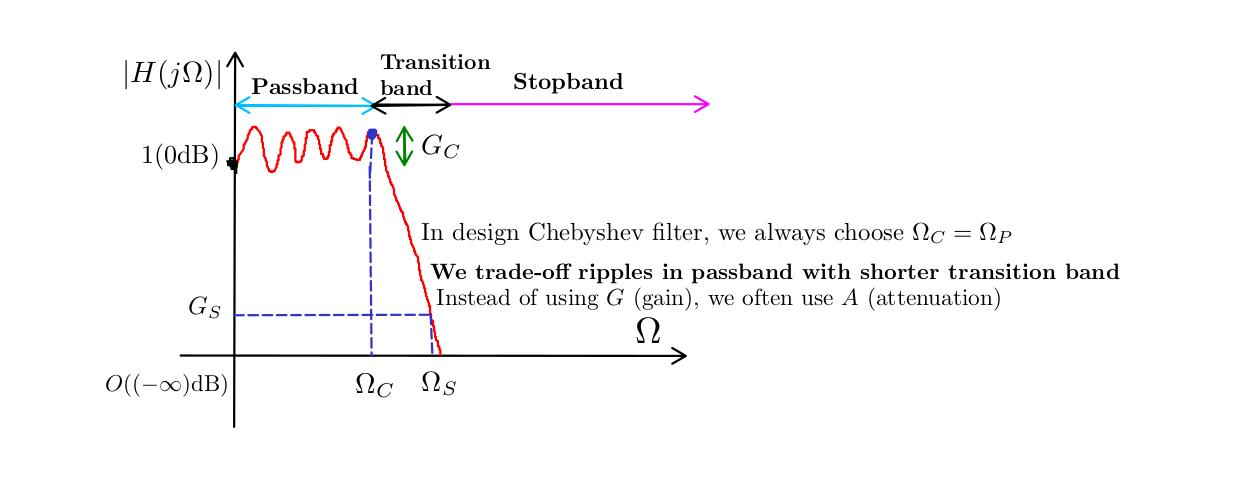
\includegraphics[width=1.1\textwidth]{15.jpg}
	\caption{Frequency response of Chebyshev LP filter}			\label{fig:re2}
		\end{figure}


\end{frame}
\begin{frame}{Thiết kế bộ lọc tương tự}
Các nhà toán học đã xấp xỉ đáp ứng tần số $|H(j\Omega)|$ của bộ lọc Chebyshev như sau:
$$|H(j\Omega)|=\frac{\sqrt{\alert{\alpha}}}{\sqrt{1+\varepsilon^2 T_{N}^2\left(\righ\frac{\Omega}{\Omega_{C}}\right)}}\Rightarrow |H^2(j\Omega)|=\frac{\alert{\alpha}}{1+\varepsilon^2 T_{N}^2\left(\righ\frac{\Omega}{\Omega_{C}}\right)}$$

	Khác với bộ lọc Butterworth, \alert{tần số cắt $\Omega_{C}$} của bộ lọc Chebyshev được định nghĩa là \textbf{tần số biên của dải thông}, mà tại vị trí này ripples bắt đầu không còn nữa, và tín hiệu dần bị suy hao do tiến vào dải chuyển tiếp. 
	  \\ \alert{Chính vì thế nên độ suy hao tại tần số cắt của bộ lọc Chebyshev hoàn toàn phụ thuộc vào gợn sóng dải thông, chứ \textbf{không cố định tại điểm 3dB}}.
	\\$T_{N}(x)$ là đa thức Chebyshev bậc $N$ được định nghĩa như sau: $$\cos(Nx)=T_{N}(\cos(x))$$
	Ví dụ:
\begin{enumerate}
	\item[1] $$\cos(x)=\cos(x)\Rightarrow T_{1}(x)=x$$
	\item[2] $$\cos(2x)=2\cos^2(x)-1\Rightarrow T_{2}(x)=2x^2-1$$
	\item[3] $$\cos(3x)=4\cos^3(x)-3\cos(x)\Rightarrow T_{3}(x)=4x^3-3x$$
	\item[4] $$\cos(4x)=8\cos^4(x)-8\cos^2(x)+1\Rightarrow T_{4}(x)=8x^4-8x^2+1$$
\end{enumerate}
\end{frame}
\begin{frame}{Thiết kế bộ lọc tương tự}
\begin{figure}[h]
	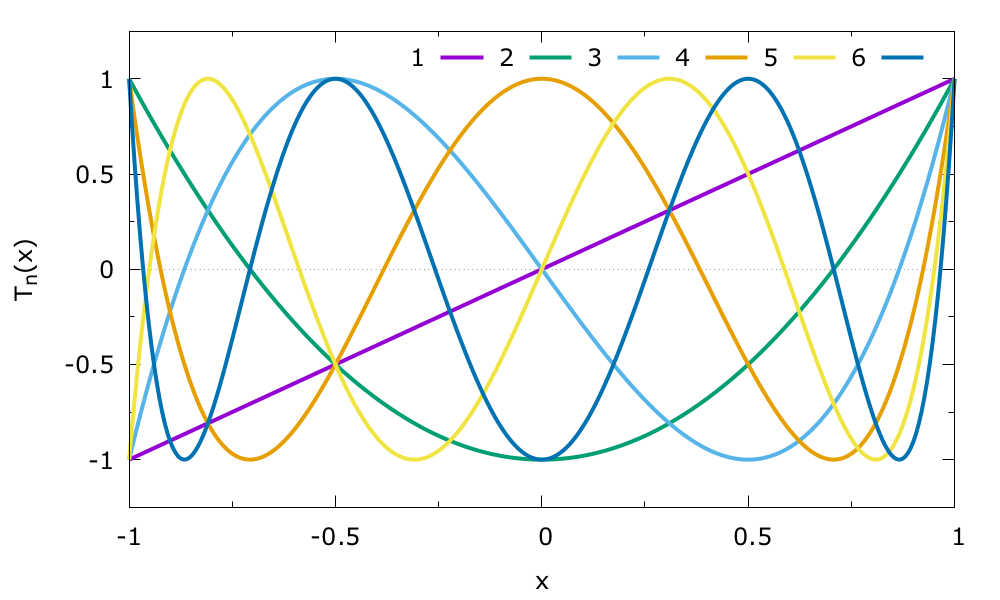
\includegraphics[width=1\textwidth]{ves_basisf-chebyshev.png}
	\caption{Chebyshev Polinomials}			\label{fig:re2}
		\end{figure}

\end{frame}
\begin{frame}{Thiết kế bộ lọc tương tự}
	Đa thức Chebyshev $T_{N}(x)$ \textbf{gợn sóng rất mạnh} với $x\in[0,1]$, và tắt gợn sóng với $x>1$. Đây cũng chính là ý nghĩa toán học của khái niệm \textbf{tần số cắt} $\Omega_{C}$. Ta có thể dễ dàng thấy rằng với $0<\Omega<\Omega_{C}$, đáp ứng tần số gợn sóng trên dải thông và $\Omega>\Omega_{C}$ thì suy hao trên dải chuyển tiếp. 
	\\ Ta quan sát dải thông của bộ lọc và đồ thị đa thức Chebyshev trong khoảng $[0,1]$, dễ thấy:
$$0\leq T_{N}^2\left(\frac{\Omega}{\Omega_{C}}\right)\leq1$$
Vậy ta thu được khoảng biến thiên của đáp ứng tần số trong dải thông:
$$\frac{\alpha}{1+\varepsilon^2}\leq |H^2(j\Omega)|\leq\alpha$$
Ta tính được độ suy hao \textbf{cực đại} (attenuation) do hiện tượng gợn sóng (ripples) gây ra trong dải thông theo thang dB:
$$\textbf{max }A_{r}=10\log_{10}\frac{\alpha}{\frac{\alpha}{1+\varepsilon^2}}=10\log_{10}(1+\varepsilon^2)$$
Ta định nghĩa khái niệm độ gợn sóng $r$ (thang dB) như sau:
$$r=\textbf{max } A_{r}=10\log_{10}(1+\varepsilon^2)\Rightarrow \varepsilon^2=10^{\frac{r}{10}}-1$$
\end{frame}
\begin{frame}{Thiết kế bộ lọc tương tự}
Ta muốn thiết kế bộ lọc có độ khuếch đại DC, tức là $$|H(0)|=1$$
Từ các đa thức Chebyshev, ta thấy:
\begin{equation*}
\begin{cases}
T^2_{N}(0)=0\quad(\text{N odd})\\
T^2_{N}(0)=1\quad(\text{N even})\\
\end{cases}
\end{equation*}
Từ dạng của đáp ứng tần số $|H^2(j\Omega)|$, ta chọn $\alpha$ theo quy tắc để thỏa mãn điều kiện khuếch đại DC:

\begin{equation*}
\begin{cases}
\alpha=1\quad(\text{N odd})\\
\alpha=\varepsilon^2+1\quad(\text{N even})\\
\end{cases}
\end{equation*}
\end{frame}
\begin{frame}{Thiết kế bộ lọc tương tự}
\begin{figure}[h]
	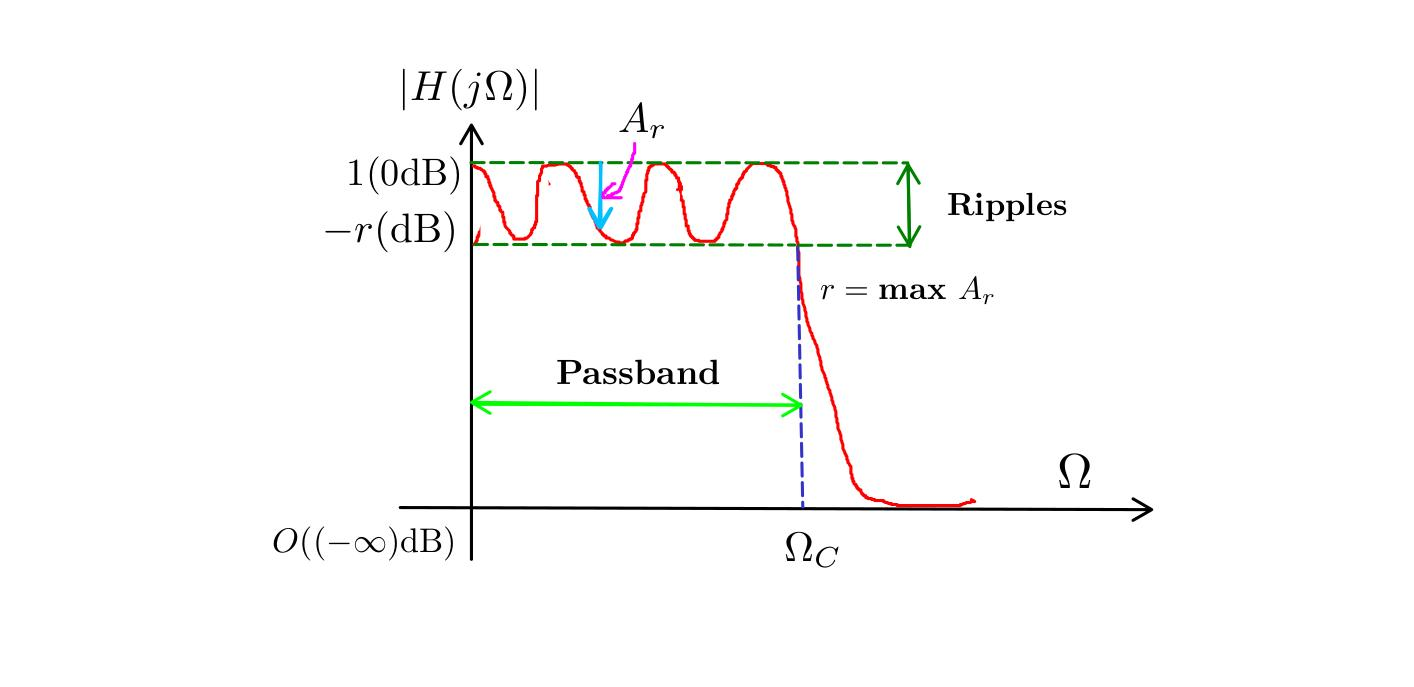
\includegraphics[width=1\textwidth]{16.jpg}
	\caption{Chebyshev LP filter N odd order}			\label{fig:re2}
		\end{figure}

\end{frame}
\begin{frame}{Thiết kế bộ lọc tương tự}
Từ công thức đa thức Chebyshev: $$\cos(Nx)=T_{N}(\cos(x))$$
Ta đặt $\cos(x)=t$, hiển nhiên $|t|\leq 1$, biến đổi tương đương ta có:
$$\cos(Nx)=T_{N}(\cos(x))\Rightarrow T_{N}(t)=\cos{(N\arccos(t))}\quad (|t|\leq 1)$$
Với $|t|>1$, ta công nhận không chứng minh: $$T_{N}(t)=\cosh(N\text{ arccosh}{(t)})\Rightarrow \alert{N=\frac{\text{arccosh}(T_{N}(t))}{\text{arccosh}(t)}}$$
\\ Ví dụ: thiết kế bộ lọc LP Chebyshev từ \textbf{4 thông số cơ bản} sau: $r, \Omega_{C}, G_{S},\Omega_{S}$
Do đã có sẵn tần số cắt $\Omega_{C}$, nên ta chỉ cần tìm bậc $N$ của bộ lọc là đủ dữ kiện thiết kế.
\begin{equation*}
\begin{split}
	G_{S}&=20\log_{10}|H(j\Omega_{S})|=10\log_{10}|H^2(j\Omega_{S})|=10\log_{10}\left(\frac{\alpha}{1+\varepsilon^2T^2_{N}\left(\frac{\Omega_{S}}{\Omega_{C}}\right)}\right)\\
	     &\approx -10\log_{10}\left(1+\varepsilon^2T^2_{N}\left(\frac{\Omega_{S}}{\Omega_{C}}\right)\right)\Rightarrow T_{N}\left(\frac{\Omega_{S}}{\Omega_{C}}\right)=\sqrt{\frac{10^{\frac{-G_{s}}{10}}-1}{\varepsilon^2}}
\end{split}
\end{equation*}
$$\Rightarrow \alert{N=\text{arccosh}\left(\sqrt{\frac{10^{\frac{-G_{s}}{10}}-1}{\varepsilon^2}}
\right)\bigg/\text{arccosh}\left(\frac{\Omega_{S}}{\Omega_{C}}\right)}$$
\end{frame}
\begin{frame}{Thiết kế bộ lọc tương tự}
Thay $A_{S}=-G_{S}$, ta thu được công thức:$$\alert{N=\text{arccosh}\left(\sqrt{\frac{10^{\frac{A_{s}}{10}}-1}{\varepsilon^2}}
\right)\bigg/\text{arccosh}\left(\frac{\Omega_{S}}{\Omega_{C}}\right)}$$
Ví dụ: thiết kế bộ lọc Chebyshev có thông số sau
	$$0<\Omega<10\text{ (rad/s)}; \quad 0<A<2.5\text{ (dB)}$$
	$$\Omega>20\text{ (rad/s)}; \quad A>23\text{ (dB)}$$
Ta xác định được 4 thông số cơ bản với giá trị tương ứng sau: 
$$\Omega_{C}=10\;, r=2.5\;, \Omega_{S}=20\;,A_{S}=23$$
Ta tìm hệ số $\varepsilon^2$: $$\varepsilon^2=10^{\frac{r}{10}}-1=0.778$$
Từ công thức trên, ta tìm được bậc $N$ của bộ lọc:
$$N=\text{arccosh}\left(\sqrt{\frac{10^{\frac{A_{s}}{10}}-1}{\varepsilon^2}}
\right)\bigg/\text{arccosh}\left(\frac{\Omega_{S}}{\Omega_{C}}\right)=2.629\Rightarrow \lceil N\rceil =3$$
Do đây là bộ lọc bậc lẻ nên ta chọn $\alpha=1$ để thỏa mãn yêu cầu độ khuếch đại DC.
\end{frame}
\begin{frame}{Thiết kế bộ lọc tương tự}
Sau khi đã xác định được đáp ứng tần số $|H(j\Omega)|$ của bộ lọc Chebyshev LP, ta hoàn toàn có thể áp dụng lại thuật toán thiết kế với bộ lọc Butterworth LP ở trên.
\\ Ta bắt đầu thiết kế từ hàm truyền bộ lọc có \alert{tần số cắt chuẩn hóa}:
$$|H_{N}^2(j\lambda)|=\frac{1}{1+\varepsilon^2 T^2_{3}(\lambda)}=\frac{1}{1+0.778(4\lambda^3-3\lambda)^2}$$
Thay $p=j\lambda$, ta thu được:
$$|H^2_{N}(j\lambda)|=\frac{1}{1+12.448\lambda^6-18.672\lambda^4+7\lambda^2}=H_{N}(p)H_{N}(-p)$$$$=\frac{1}{-12.448p^6-18.672p^4-7p^2+1}$$
Bằng phương pháp giải căn bậc 2 mũ phức tương tự như phần bộ lọc Butterworth, ta tìm ra các nghiệm cực thỏa mãn $\Re{(p)}<0$ sau:
\begin{equation*}
\begin{cases}
	p_{1}=-0.33\\
	p_{2}=-0.926\angle 1.3919\\
	p_{3}=-0.926\angle -1.3919\\
\end{cases}
\end{equation*}
Áp dụng định lý Viete đảo, ta tìm được phương trình nghiệm cực của bộ lọc chuẩn hóa là:
$$(p+0.33)(p^2+0.3295p+0.8574)$$
\end{frame}
\begin{frame}{Thiết kế bộ lọc tương tự}
Vậy ta thu được hàm truyền của bộ lọc chuẩn hóa:
$$H_{N}(p)=\frac{\alert{0.33 . 0.8574}}{(p+0.33)(p^2+0.395p+0.8574)}=\frac{0.2829}{(p+0.33)(p^2+0.3295p+0.8574)}$$
Tách mẫu thức, ta thu được:
$$H_{N}(p)=\frac{0.2829}{p^3+0.6595p^2+0.9661p+0.2829}$$
Ta đổi biến: $$p=\frac{s}{\Omega_{C}}=\frac{s}{10}$$
Và thu được hàm truyền của bộ lọc cần tìm:
$$H(s)=\frac{282.9}{s^3+6.595s^2+96.91s+282.9}$$
\end{frame}
\begin{frame}{Thiết kế bộ lọc tương tự}
\begin{block}{Thuật toán thiết kế bộ lọc Chebyshev LP}
\begin{enumerate}
	\item[1] Xác định hằng số $\varepsilon^2$ và bậc $N$ của bộ lọc cần thiết kế
	\item[2] Xác định hằng số $\alpha$, và tìm đáp ứng tần số của bộ lọc có \textbf{tần số cắt chuẩn hóa}
		$$|H_{N}^2(j\lambda)|=\frac{\alpha}{1+\varepsilon^2 T^2_{N}(\lambda)}$$
	\item[3] Thay $p=j\lambda$, tìm đa thức cực và xác định hàm truyền của bộ lọc có \textbf{tần số cắt chuẩn hóa}:
		$$H_{N}(p)=\frac{\prod_{k=0}^{M}(-p_{k})}{\prod_{k=0}^{M}(s-p_{k})}\quad(\Re{(p_{k})}<0)$$
	\item[4] Đổi biến: $$p=\frac{s}{\Omega_{C}}\Rightarrow H(s)=H_{N}\left(\frac{s}{\Omega_{C}}\right)$$ Ta thu được hàm truyền $H(s)$ của bộ lọc cần tìm.
\end{enumerate}
\end{block}
\end{frame}
\begin{frame}{Thiết kế bộ lọc tương tự}
\subsection{Thiết kế bộ lọc BP}
\begin{itemize}
	\item Thiết kế bộ lọc BP
\end{itemize}
\subsubsection{Ý tưởng thiết kế bộ lọc BP}
\begin{itemize}
	\item[-] Ý tưởng thiết kế bộ lọc BP 
\end{itemize}
\begin{figure}[h]
	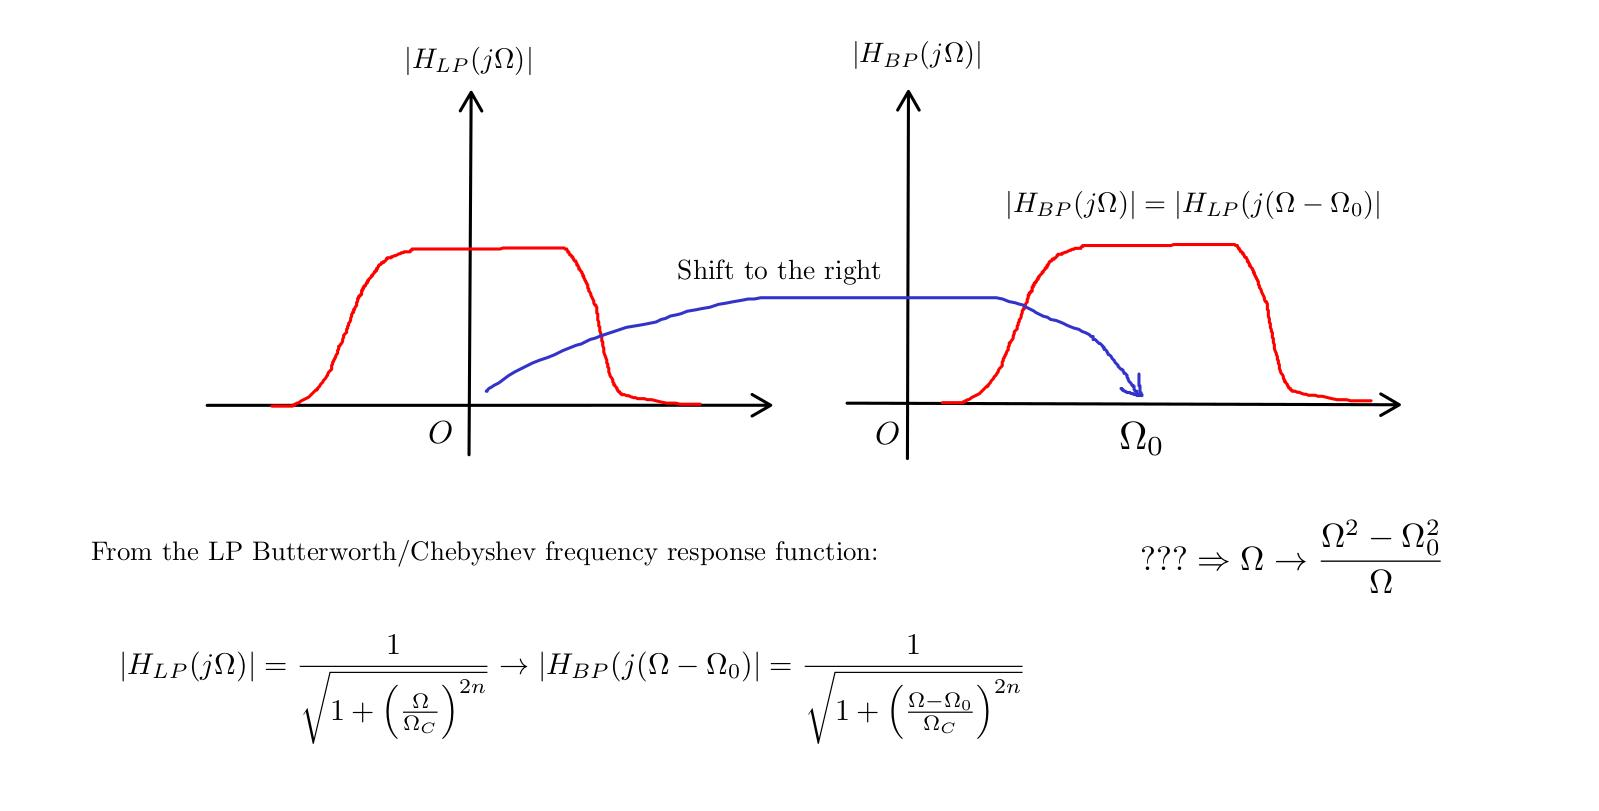
\includegraphics[width=1\textwidth]{17.jpg}
	\caption{Idea of BP filter design}			\label{fig:re2}
		\end{figure}

\end{frame}
\begin{frame}{Thiết kế bộ lọc tương tự}
Đối với bộ lọc LP \alert{có tần số cắt thường}, ta quy ước:
\begin{enumerate}
	\item[1] Kí hiệu tần số góc: $\lambda$
	\item[2] Kí hiệu biến Laplace: $p$
	\item[3] Kí hiệu hàm truyền: $H_{LP}(p)$
\end{enumerate}
Đối với bộ lọc BP, ta quy ước:

\begin{enumerate}
	\item[1] Kí hiệu tần số góc: $\Omega$
	\item[2] Kí hiệu biến Laplace: $s$
	\item[3] Kí hiệu hàm truyền: $H_{BP}(s)$
\end{enumerate}
\end{frame}
\begin{frame}{Thiết kế bộ lọc tương tự}
\begin{figure}[h]
	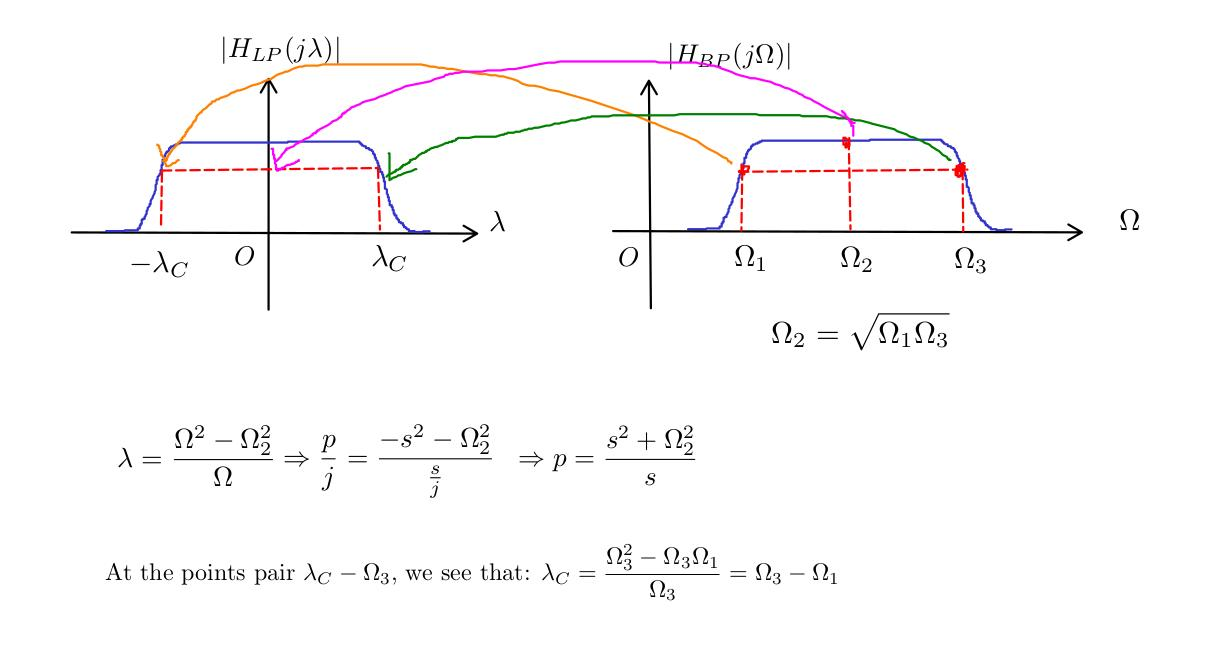
\includegraphics[width=1\textwidth]{18.jpg}
	\caption{Mapping frequency in designing BP filter}			\label{fig:re2}
		\end{figure}


\end{frame}
\begin{frame}{Thiết kế bộ lọc tương tự}
\subsubsection{Thuật toán thiết kế bộ lọc BP}
\begin{itemize}
	\item[-] Thuật toán thiết kế bộ lọc BP
\end{itemize}
\begin{block}{Thuật toán thiết kế bộ lọc BP}
\begin{enumerate}
	\item[1] Xác định \textbf{tần số trung bình hình học} $\Omega_{2}$ của bộ lọc BP: $$\Omega_{2}=\sqrt{\Omega_{1}\Omega_{3}}$$
	Với $\Omega_{1},\Omega_{3}$ là \textbf{tần số cắt} ở hai phía của dải thông (do bộ lọc BP đối xứng tại vị trí $\Omega_{2}$).
\item[2] Ánh xạ toàn bộ tần số bộ lọc BP sang bộ lọc LP bằng công thức: $$\lambda=\frac{\Omega^2-\Omega_{2}^2}{\Omega}$$
\item[3] Thiết kế bộ lọc LP có hàm truyền $H_{LP}(p)$ tương ứng từ dữ liệu thu được ở bước trên.
\item[4] Đổi biến: $$p=\frac{s^2+\Omega_{2}^2}{s}$$ 
	Ta thu được hàm truyền $H_{BP}(s)$ của bộ lọc cần tìm
\end{enumerate}
\end{block}
\end{frame}
\begin{frame}{Thiết kế bộ lọc tương tự}
Ví dụ: thiết kế bộ lọc BP thỏa mãn đặc tả sau:
$$\Omega<10\;\text{(rad/s)};\quad A>20\text{ (dB)}$$
$$20<\Omega<40\;\text{(rad/s)};\quad 0<A<2\text{ (dB)}$$
$$\Omega>50\;\text{(rad/s)};\quad A>20\text{ (dB)}$$
\textbf{Lưu ý: khi $A_{P}=3$ ta có thể chọn cả 2 loại bộ lọc Chebyshev và Butterworth để thiết kế, nhưng nếu $A_{P}\neq3$ ta chỉ có thể chọn bộ lọc Chebyshev.}
\\Trong đặc tả trên, ta thấy $A_{P}\neq3$, nên ta chọn bộ lọc Chebyshev có: $$r=\textbf{max }A_{P}=2\text{ (dB)}$$
Ta phác họa đáp ứng biên độ của bộ lọc BP trên đồ thị:
\begin{figure}[h]
	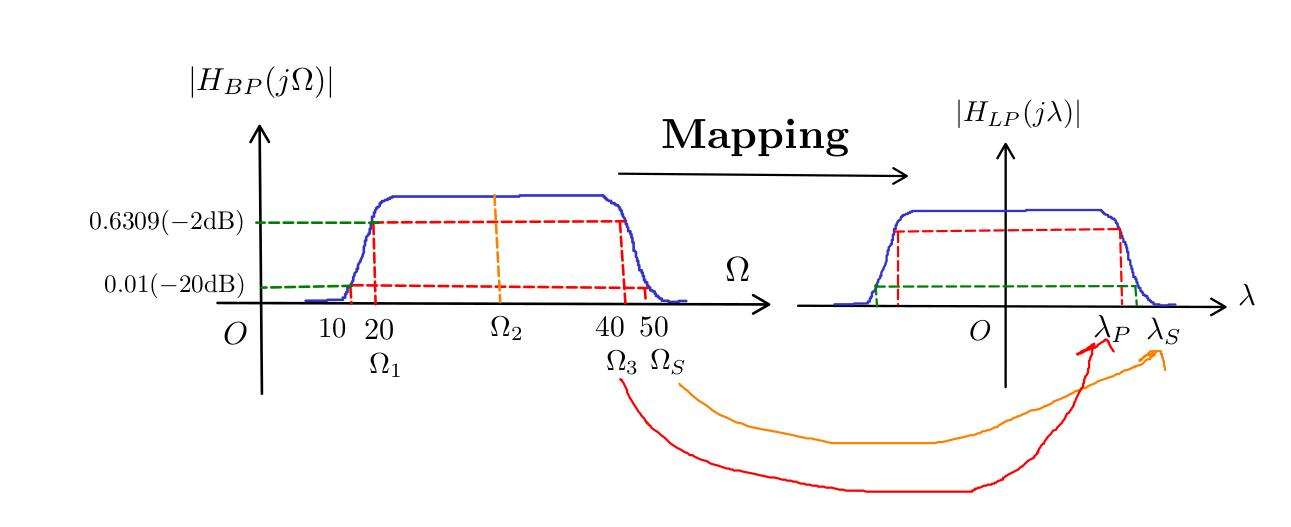
\includegraphics[width=0.8\textwidth]{19.jpg}
	\caption{Mapping frequency algorithm}			\label{fig:re2}
		\end{figure}

\end{frame}
\begin{frame}{Thiết kế bộ lọc tương tự}
Với $\Omega_{2}=\sqrt{\Omega_{1}\Omega_{3}}=28.28$ (rad/s),
ta lần lượt ánh xạ các tần số: $$\lambda=\frac{\Omega^2-\Omega_{2}^2}{\Omega}\Rightarrow \lambda_{P}=\frac{\Omega_{3}^2-\Omega_{2}^2}{\Omega_{3}}=20;\;\lambda_{S}=\frac{\Omega_{S}^2-\Omega_{2}^2}{\Omega_{S}}=34$$
 Ta thiết kế bộ lọc Chebyshev LP hàm truyền $H_{LP}(p)$ có đặc tả:
$$\lambda<20\;\text{(rad/s)};\quad A<2\text{ (dB)}$$
$$\lambda>34\;\text{(rad/s)};\quad A>20\text{ (dB)}$$
Bằng phương pháp thiết kế đã được trình bày rất kĩ ở trên, ta tìm được bậc bộ lọc $N=3$, và thu được hàm truyền:
$$H_{LP}(p)=\frac{0.201}{p^3+0.133p^2+3p+0.201}$$
Đổi biến $$p=\frac{s^2+800}{s}$$
Ta thu được hàm truyền $H_{BP}(s)$ của bộ lọc thông dải cần tìm.
\end{frame}
\begin{frame}{Thiết kế bộ lọc tương tự}
\subsection{Thiết kế bộ lọc BS}
\begin{itemize}
	\item Thiết kế bộ lọc BS
\end{itemize}
\subsubsection{Ý tưởng thiết kế bộ lọc BS}
\begin{itemize}
	\item[-] Ý tưởng thiết kế bộ lọc BS
\end{itemize}
\begin{figure}[h]
	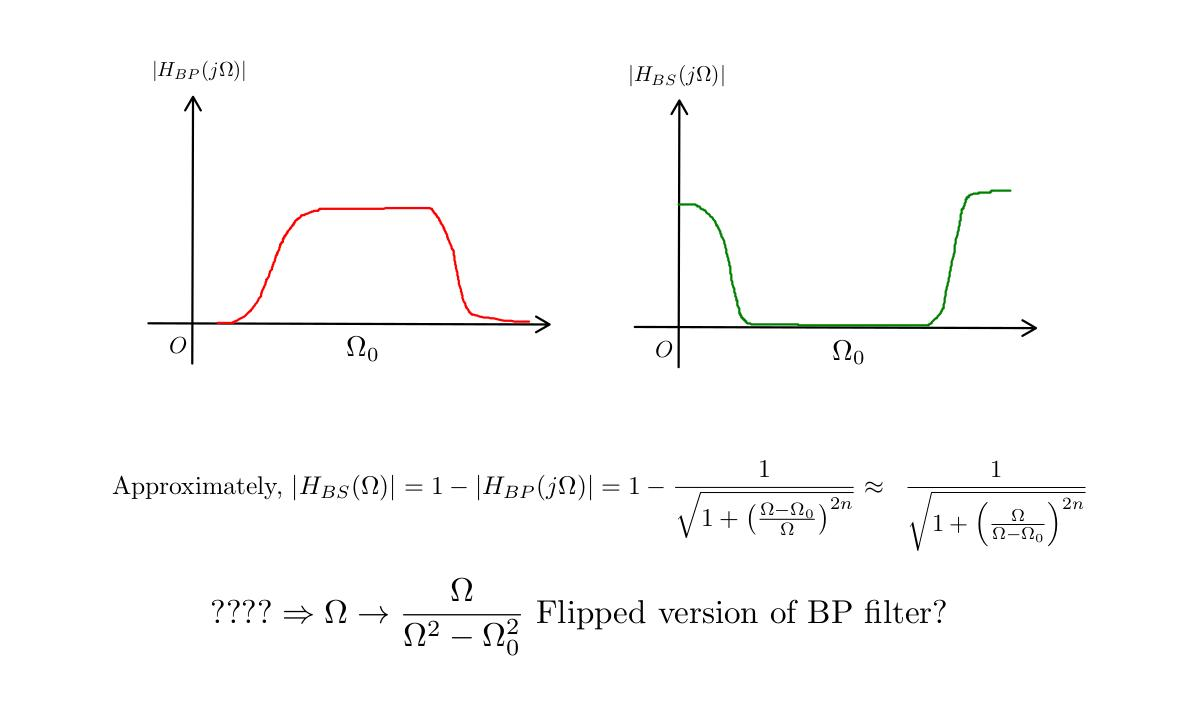
\includegraphics[width=1\textwidth]{20.jpg}
	\caption{Idea of BS filter design}			\label{fig:re2}
		\end{figure}
\end{frame}
\begin{frame}{Thiết kế bộ lọc tương tự}
\begin{figure}[h]
	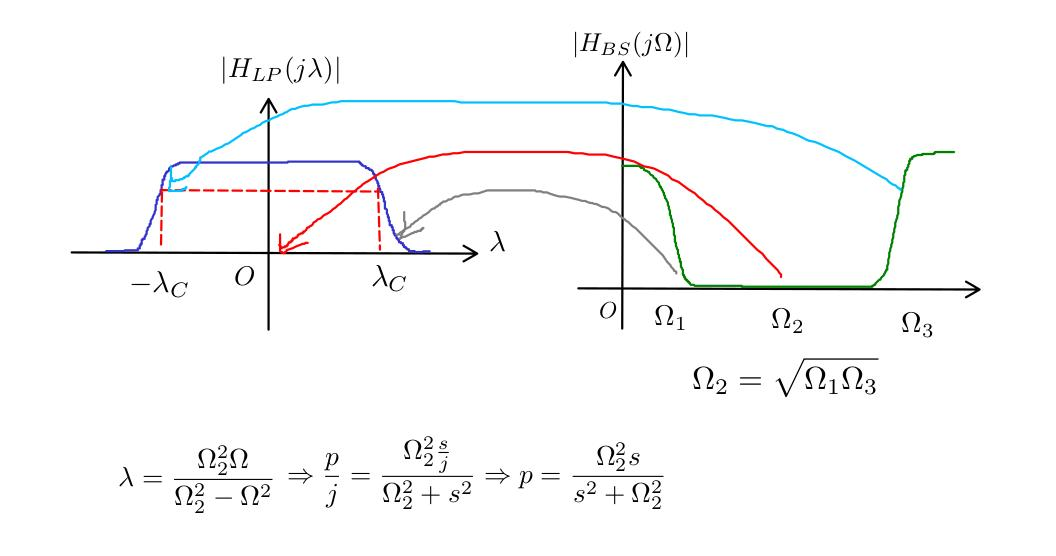
\includegraphics[width=1\textwidth]{21.jpg}
	\caption{Mapping frequency in designing BS filter}			\label{fig:re2}
		\end{figure}

\end{frame}
\begin{frame}{Thiết kế bộ lọc tương tự}
\subsubsection{Thuật toán thiết kế bộ lọc BS}
\begin{itemize}
	\item[-] Thuật toán thiết kế bộ lọc BS
\end{itemize}
\begin{block}{Thuật toán thiết kế bộ lọc BS}
\begin{enumerate}
	\item[1] Xác định \textbf{tần số trung bình hình học} $\Omega_{2}$ của bộ lọc BS: $$\Omega_{2}=\sqrt{\Omega_{1}\Omega_{3}}$$
	Với $\Omega_{1},\Omega_{3}$ là \textbf{tần số cắt} ở hai phía của dải triệt (do bộ lọc Bs đối xứng tại vị trí $\Omega_{2}$).
\item[2] Ánh xạ toàn bộ tần số bộ lọc BS sang bộ lọc LP bằng công thức: $$\alert{\lambda=\frac{\Omega_{2}^2\Omega}{\Omega_{2}^2-\Omega^2}}$$
\item[3] Thiết kế bộ lọc LP có hàm truyền $H_{LP}(p)$ tương ứng từ dữ liệu thu được ở bước trên.
\item[4] Đổi biến: $$\alert{p=\frac{\Omega_{2}^2s}{s^2+\Omega_{2}^2}}$$ 
	Ta thu được hàm truyền $H_{BS}(s)$ của bộ lọc cần tìm
\end{enumerate}
\end{block}
\end{frame}
\begin{frame}{Thiết kế bộ lọc tương tự}
 Ví dụ: thiết kế bộ lọc thỏa mãn đặc tả:
$$\Omega<10\;\text{(rad/s)};\quad A<3\text{ (dB)}$$
$$20<\Omega<40\;\text{(rad/s)};\quad A>20\text{ (dB)}$$
$$\Omega>50\;\text{(rad/s)};\quad A<3\text{ (dB)}$$
Do $A_{P}=3$, nên ta có thể chọn cả 2 loại bộ lọc Butterworth và Chebyshev để thiết kế, ở đây ta chọn bộ lọc Butterworth.
\\ Ta phác họa đáp ứng tần số của bộ lọc:
\begin{figure}[h]
	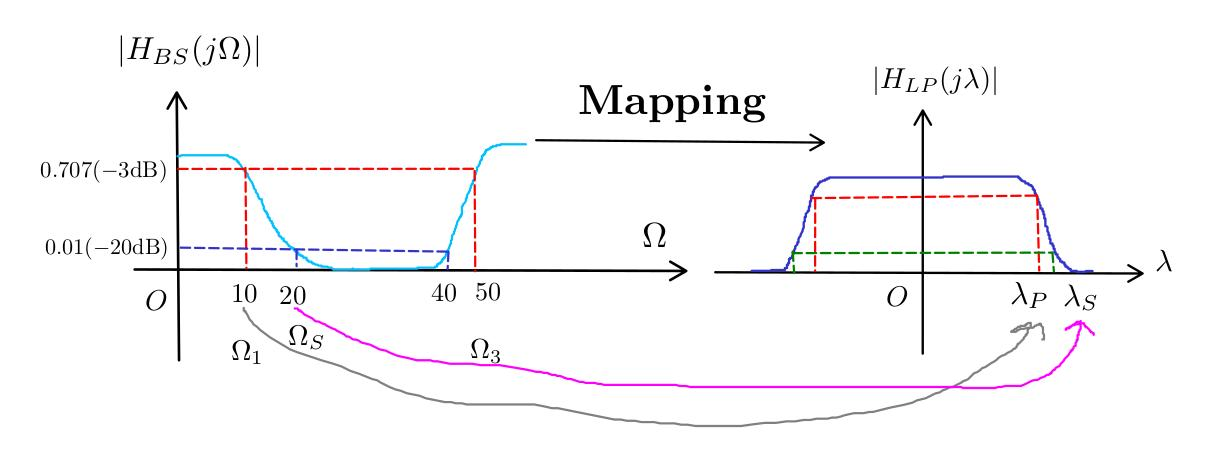
\includegraphics[width=1\textwidth]{22.jpg}
	\caption{Mapping frequency algorithm}			\label{fig:re2}
		\end{figure}


\end{frame}
\begin{frame}{Thiết kế bộ lọc tương tự}
Hiển nhiên, ta thấy lúc này: $$\Omega_{2}=\sqrt{\Omega_{1}\Omega_{3}}=\sqrt{10.50}=22.36$$ Ta ánh xạ các tần số theo công thức:
$$\lambda=\frac{\Omega_{2}^2\Omega}{\Omega_{2}^2-\Omega^2}\Rightarrow \lambda_{P}=\frac{\Omega_{2}^2\Omega_{1}}{\Omega_{2}^2-\Omega_{1}^2}=12.5;\;\lambda_{S}=\frac{\Omega_{2}^2\Omega_{S}}{\Omega_{2}^2-\Omega_{S}^2}=100.02$$
Tiếp theo, ta thiết kế bộ lọc LP Butterworth  với các thông số $\lambda_{P}=12.5,\;\lambda_{S}=100.02\; ,A_{P}=3\; ,A_{S}=20$. \\Với thuật toán thiết kế đã được trình bày rất kĩ ở trên, ta thu được hàm truyền:
$$H_{LP}(p)=\frac{156.621}{p^2+17.6986p+156.621}$$
Đổi biến: 
$$p=\frac{\Omega_{2}^2s}{s^2+\Omega_{2}^2}=\frac{500s}{s^2+500}$$
Ta thu được hàm truyền $H_{BS}(s)$ của bộ lọc chặn dải cần tìm.
\end{frame}
\begin{frame}{Thiết kế bộ lọc tương tự}
\subsection{Thiết kế bộ lọc HP}
\begin{itemize}
	\item Thiết kế bộ lọc HP
\end{itemize}
\subsubsection{Ý tưởng thiết kế bộ lọc HP}
\begin{itemize}
	\item[-] Ý tưởng thiết kế bộ lọc HP
\end{itemize}
\begin{figure}[h]
	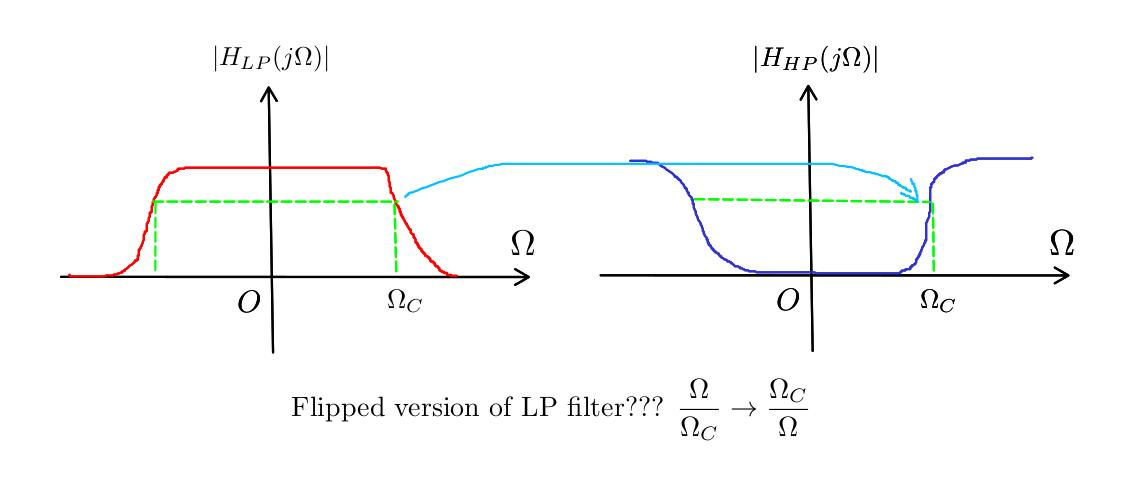
\includegraphics[width=1\textwidth]{23.jpg}
	\caption{Idea of HP filter design}			\label{fig:re2}
		\end{figure}

\end{frame}
\begin{frame}{Thiết kế bộ lọc tương tự}
\begin{figure}[h]
	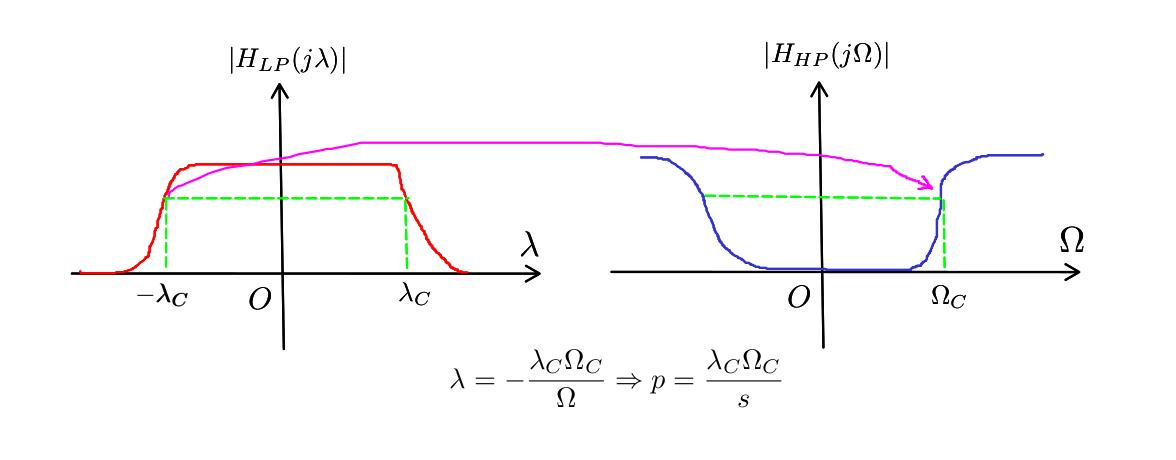
\includegraphics[width=1\textwidth]{24.jpg}
	\caption{Mapping frequency in designing HP filter}			\label{fig:re2}
		\end{figure}


\end{frame}
\begin{frame}{Thiết kế bộ lọc tương tự}
	\begin{itemize}
		\item[-] Thuật toán thiết kế bộ lọc HP
	\end{itemize}
\begin{block}{Thuật toán thiết kế bộ lọc HP}
	\begin{enumerate}
		\item[1] Với bộ lọc HP, ta luôn có: $$\alert{\lambda_{C}=\Omega_{C}}$$ Ánh xạ toàn bộ tần số bộ lọc HP sang LP bằng công thức:
			$$\lambda=-\frac{\lambda_{C}\Omega_{C}}{\Omega}$$
		\item[2] Thiết kế bộ lọc thông thấp có hàm truyền $H_{LP}(p)$. 
		\item[3] Đổi biến: $$p=\frac{\lambda_{C}\Omega_{C}}{s}$$ Ta thu được hàm truyền $H_{HP}(s)$ của bộ lọc cần tìm.
	\end{enumerate}
\end{block}
\subsubsection{Thuật toán thiết kế bộ lọc HP}
\end{frame}
\begin{frame}{Thiết kế bộ lọc tương tự}
Ví dụ: thiết kế bộ lọc tương tự với đặc tả sau:
	$$0<\Omega<10\text{ (rad/s)}; \quad A>23\text{ (dB)}$$
	$$\Omega>20\text{ (rad/s)}; \quad 0<A<3\text{ (dB)}$$
Ta chọn thiết kế bằng bộ lọc Chebyshev và phác họa đáp ứng biên độ của bộ lọc HP trên đồ thị:
\begin{figure}[h]
	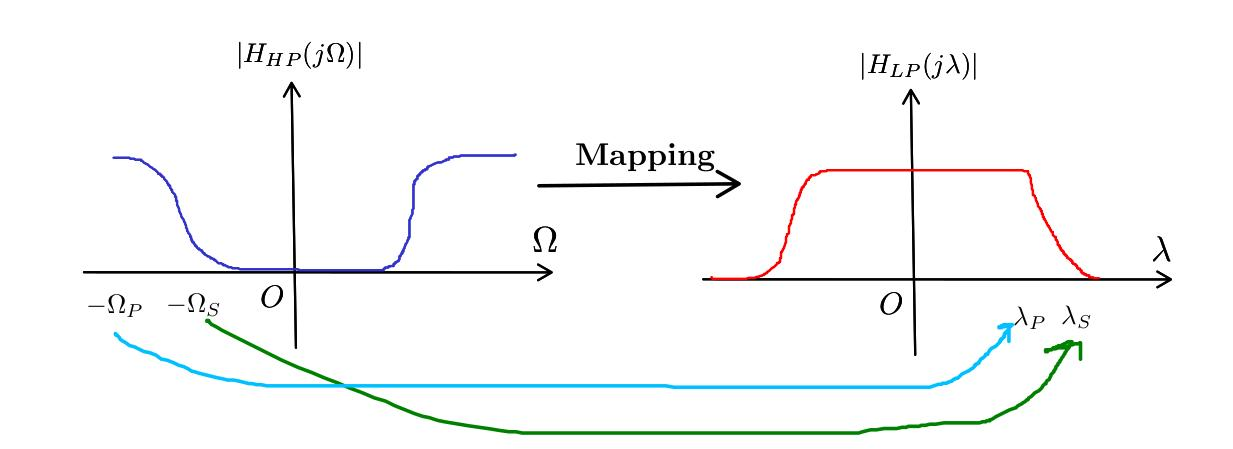
\includegraphics[width=1\textwidth]{25.jpg}
	\caption{Mapping frequency in designing HP filter}			\label{fig:re2}
		\end{figure}

\end{frame}
\begin{frame}{Thiết kế bộ lọc tương tự}
Từ thông số đề bài $\Omega_{S}=10,\;\Omega_{P}=20$, ta dùng công thức chuyển đổi tần số để ánh xạ sang bộ lọc LP tương ứng:
$$\lambda_{C}=\Omega_{\alert{P}}=\Omega_{\alert{C}}=20$$
$$\lambda_{S}=-\frac{\lambda_{C}\Omega_{C}}{\alert{-\Omega_{S}}}=40$$
Vậy ta thiết kế bộ lọc LP Chebyshev với đặc tả: $\lambda_{C}=20,\;\lambda_{S}=40,\;r=3,\;A_{S}=23$
\\ Sử dụng phương pháp thiết kế đã được trình bày rất kĩ ở trên, ta thu được:
$$H_{LP}(p)=\frac{2004.754}{p^3+11.944p^2+371.339p+2004.754}$$
Đổi biến: $$p=\frac{400}{s}$$
Ta thu được hàm truyền của bộ lọc $H_{HP}(p)$ cần tìm.
\end{frame}
\begin{frame}[fragile]{Thiết kế bộ lọc tương tự}
\subsection{Thực hành}
\begin{itemize}
	\item Thực hành
\end{itemize}
Ta sẽ sử dụng phần mềm GNU Octave để thiết kế bộ lọc LP tương tự (Matlab hỗ trợ thiết kế cả 4 loại bộ lọc):
\begin{verbatim}
	[n On]=buttord(Op,Os,Ap,As,'s'); % Butterworth LP filter
	[b a]=butter(n, On,'s');
	[n On]=cheb1ord(Op,Os,Ap,As,'s'); % Chebyshev LP filter
	[b a]=cheby1(n,Ap,On,'s'); 
	w=linspace(starting_point,ending_point,number_of_points);
	freqs(b,a,w) % Plot magnitude and phase spectrum of analog filter
\end{verbatim}
Các bạn có thể áp dụng đoạn code này để kiếm tra lại đáp án các bài tập thiết kế bộ lọc.
\end{frame}
\begin{frame}{Thiết kế bộ lọc số}
	\section{Thiết kế bộ lọc số}
\begin{itemize}
	\item Ý tưởng thiết kế bộ lọc số
\end{itemize}
\subsection{Ý tưởng thiết kế bộ lọc số}
Bộ lọc số được thiết kế từ bộ lọc tương tự, trên cơ sở liên hệ chặt chẽ giữa biến đổi Laplace và Z. Ở môn học tiên quyết \alert{Tín hiệu và hệ thống}, ta đã tìm hiểu về hai phép biến đổi này rời rạc nhau; bây giờ ta muốn chỉ ra mối liên hệ giữa chúng làm tiền đề cho \textbf{thuật toán thiết kế bộ lọc số}.
\\Ta xét biến đổi Laplace của tín hiệu rời rạc sau:
\begin{equation*}
\begin{split}
	x[n]&=x(nT_{0})=x(t)\sum_{n=-\infty}^{+\infty}\delta(t-nT_{0})\\
\Rightarrow \mathscr{L}\left(x(nT_{0})\right)&=\mathscr{L}\left(x(t)\sum_{n=-\infty}^{+\infty}\delta(t-nT_{0})\right)=\int_{-\infty}^{+\infty}\left(x(t)\sum_{n=-\infty}^{+\infty}\delta(t-nT_{0})\right)e^{-st}dt\\
					     &=\sum_{n=-\infty}^{+\infty}x(t)\left(\int_{-\infty}^{+\infty}\delta(t-nT_{0})e^{-st}dt\right)=\sum_{n=-\infty}^{+\infty}x(t)\alert{e^{-nsT_{0}}}
\end{split}
\end{equation*}
Ta đặt $z=e^{sT_{0}}$, thu được phương trình chỉ ra mối quan hệ giữa biến đổi Laplace và Z. Chúng ta sẽ phát triển thuật toán thiết kế các loại bộ lọc số dựa trên phương trình này.
\end{frame}
\begin{frame}{Thiết kế bộ lọc số}
\subsection{Phương pháp đáp ứng xung bất biến và bậc thang}
\begin{itemize}
	\item Phương pháp đáp ứng xung bất biến và bậc thang
\end{itemize}
Đây là 2 phương pháp \textbf{không phổ biến, sai số lớn và kém chính xác} khi thiết kế bộ lọc IIR, thế nên chúng ta chỉ cần nhớ 2 công thức sau để đi thi:
\begin{enumerate}
	\item[1] Công thức đáp ứng xung bất biến:
		$$H(s)=\sum\frac{c_{i}}{s-\lambda_{i}}\to H(z)=\sum\frac{c_{i}T_{s}}{1-e^{\lambda_{i}T_{s}}z^{-1}}$$
	\item[2] Công thức đáp ứng xung bậc thang:

		$$H(s)=\sum\frac{c_{i}}{s-\lambda_{i}}\to H(z)=\sum\frac{1}{\lambda_{i}}\frac{c_{i}(e^{\lambda_{i}T_{s}}-1)z^{-1}}{1-e^{\lambda_{i}T_{s}}z^{-1}}$$
\end{enumerate}
\begin{block}{Thuật toán thiết kế bộ lọc số bằng phương pháp xung bất biến/bậc thang}
\begin{enumerate}
	\item[1] Chuyển các tần số từ miền số sang miền tương tự:
		$$\omega=2\pi\frac{F}{F_{sam}}
		\Rightarrow\Omega=\frac{\omega}{T_{sam}}=\omega F_{sam}=2\pi F$$
	Với $\omega,F$ là \textbf{các tần số trong miền số}, $F_{sam}$ là \textbf{tần số lấy mẫu}.
	\item[2] Thiết kế bộ lọc tương tự dựa theo kết quả tính toán từ bước 1.
	\item[3] Sử dụng công thức đáp ứng xung bất biến hoặc xung bậc thang để chuyển đổi bộ lọc tương tự về bộ lọc số.
\end{enumerate}
\end{block}
\end{frame}
\begin{frame}{Thiết kế bộ lọc số}
\subsection{Phương pháp song tuyến tính}
\begin{itemize}
	\item Phương pháp song tuyến tính
\end{itemize}
\textbf{Phương pháp song tuyến tính} là trọng tâm của thuật toán thiết kế bộ lọc số. Các phần mềm mô phỏng như GNU Octave/Matlab đều thiết kế bộ lọc dựa trên phương pháp này.
\\ Từ biểu thức liên hệ giữa biến đổi Laplace và Z:
\begin{equation*}
\begin{split}
	z=e^{sT_{0}}&\Rightarrow z=\frac{e^{\frac{sT_{0}}{2}}}{e^{-\frac{sT_{0}}{2}}}=\frac{1+\frac{sT_{0}}{2}}{1-\frac{sT_{0}}{2}}=\frac{s+\frac{2}{T_{0}}}{-s+\frac{2}{T_{0}}}\\
		    &\Rightarrow z\left(-s+\frac{2}{T_{0}}\right)=s+\frac{2}{T_{0}}\Rightarrow s(z+1)=\frac{2}{T_{0}}(z-1)\\
		    &\Rightarrow \alert{s=\frac{2}{T_{0}}\frac{1-z^{-1}}{1+z^{-1}}=C\frac{1-z^{-1}}{1+z^{-1}}}\\
	z=\frac{s+\frac{2}{T_{0}}}{-s+\frac{2}{T_{0}}}&\Rightarrow e^{j\omega}=\frac{1+j\Omega\frac{T_{0}}{2}}{1-j\Omega\frac{T_{0}}{2}}\Rightarrow j\Omega=\frac{2}{T_{0}}\frac{1-e^{j\omega}}{1+e^{j\omega}}=\frac{2}{T_{0}}\frac{(1-e^{j\omega})(1+e^{-j\omega})}{(1+e^{j\omega})(1+e^{-j\omega})}\\
	\Rightarrow& \alert{\Omega=\frac{2}{T_{0}}\tan\left(\frac{\omega}{2}\right)=C\tan\left(\frac{\omega}{2}\right)}
\end{split}
\end{equation*}
Dễ thấy hằng số $C$ chính là \textbf{trái tim của phép biến đổi song tuyến tính}.
Ta có thể chọn: $$C=\frac{2}{T_{0}}$$
hay $C$ là bất cứ giá trị nào khác để \alert{ánh xạ tần số giữa miền thời gian liên tục và miền thời gian rời rạc.}
\end{frame}
\begin{frame}{Thiết kế bộ lọc số}
Nếu ta chọn hằng số: $$C=\frac{2}{T_{0}}$$
Dạng đáp ứng biên độ giữa bộ lọc tương tự và bộ lọc số tương đối giống nhau về dáng điệu đồ thị, nhưng ta không biết thêm bất cứ thông tin nào khác nữa. Ta cần tìm phương án chọn $C$ khác.
\\  Ta giới thiệu khái niệm "tần số số" mới được định nghĩa: $$v=\frac{F}{F_{N}}$$
Đây chỉ là khái niệm "tần số số" theo quy ước của Matlab, ở \alert{Chương 5} ta sẽ quy ước: $$v=\frac{F}{F_{sam}}$$
Hiển nhiên ta thấy rất rõ ý nghĩa vật lý của "tần số số" là "mọi tần số trong miền số không bao giờ vượt qua giá trị tần số Nyquist" (đã được thảo luận ở \alert{Chương 1}).
\end{frame}
\begin{frame}{Thiết kế bộ lọc số}
\begin{itemize}
	\item[-] Thiết kế bộ lọc LP
\end{itemize}
\\ Đối với bộ lọc tương tự LP \alert{tần số cắt chuẩn hóa}:
\begin{enumerate}
	\item[1] Kí hiệu tần số góc: $\lambda$
	\item[2] Kí hiệu biến Laplace: $p$
	\item[3] Kí hiệu hàm truyền: $H_{LP,N}(p)$
\end{enumerate}

\\ Đối với bộ lọc số LP:
\begin{enumerate}
	\item[1] Kí hiệu tần số góc: $\omega$
	\item[2] Kí hiệu tần số $F$, tần số Nyquist $F_{N}$, tần số lấy mẫu $F_{sam}$
	\item[3] Kí hiệu tần số số (theo quy ước Matlab): $v$
	\item[4] Kí hiệu biến Z: $z$
	\item[5] Kí hiệu hàm truyền: $H_{LP}(z)$
\end{enumerate}
Ta viết lại 2 công thức chuyển đổi giữa miền liên tục và miền số (liên hệ giữa biến đổi Laplace và Z):
$$\alert{p=C\frac{1-z^{-1}}{1+z^{-1}}}$$
$$\Omega=C\tan\left(\frac{\omega}{2}\right)=C\tan{\left(\frac{2\pi F}{2F_{sam}}\right)}=C\tan{\left(\frac{\pi F}{F_{sam}}\right)}=\alert{C\tan{\left(\frac{\pi v}{2}\right)}}$$
$$\Rightarrow \alert{C=\Omega\cot{\left(\frac{\pi v}{2}\right)}}$$
\end{frame}
\begin{frame}{Thiết kế bộ lọc số}
Ta chọn $C$ sao cho \textbf{tần số cắt trong miền số ánh xạ tới tần số cắt trong miền tương tự}, tức là: $$v_{C}\to\Omega_{C}$$
Nếu ta chọn bộ lọc LP trong miền tương tự để ánh xạ tới là bộ lọc có tần số cắt chuẩn hóa:
$$\alert{v_{C}\to\lambda_{C}=1\text{ (rad/s) }}$$
Vậy ta thu được công thức tìm hằng số $C$:
$$\alert{C=\lambda_{C}\cot{\left(\frac{\pi v_{C}}{2}\right)}=\cot{\left(\frac{\pi v_{C}}{2}\right)}}$$
\begin{figure}[h]
	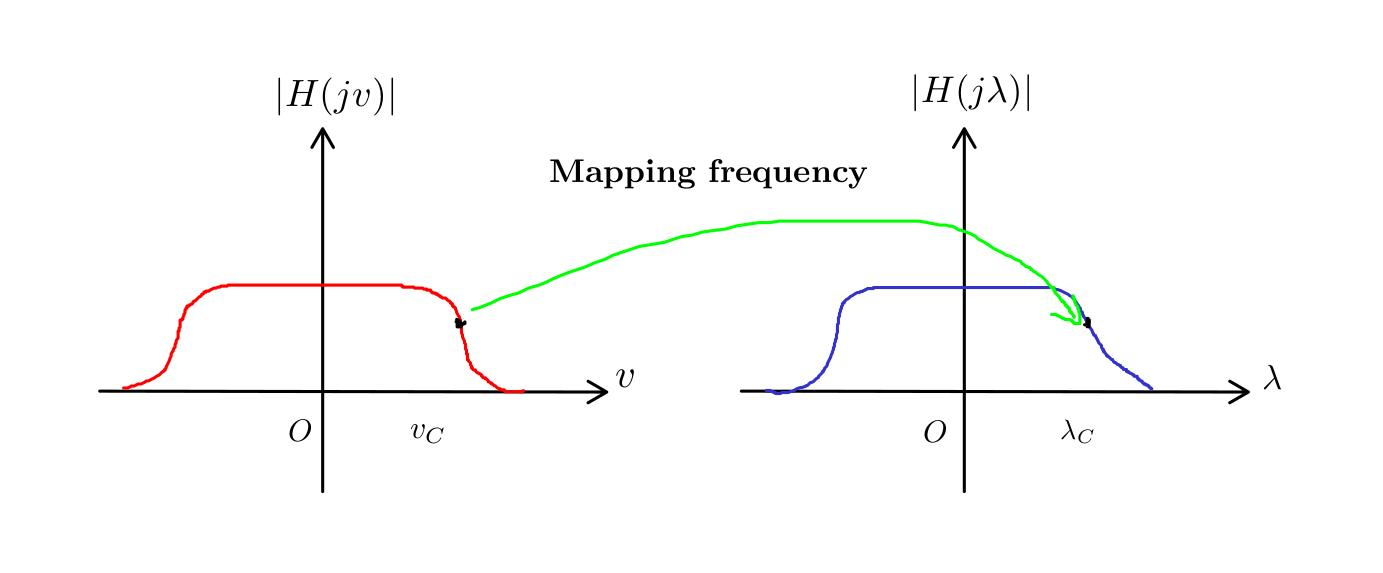
\includegraphics[width=0.8\textwidth]{26.jpg}
	\caption{Designing digital LP filter}			\label{fig:re2}
		\end{figure}


\end{frame}
\begin{frame}{Thiết kế bộ lọc số}
	\begin{block}{Thuật toán thiết kế bộ lọc LP số}
	\begin{enumerate}
	\item[1] Chuyển các tần số trong miền số về các tần số số $v$:
		$$\alert{v=\frac{F}{F_{N}}}$$
	\item[2] Xác định tần số cắt số $v_{C}$, và tính hằng số $C$ theo công thức:
$$\alert{C=\cot{\left(\frac{\pi v_{C}}{2}\right)}}$$
\item[3] Ánh xạ từng tần số trong miền số sang miền tương tự với hằng số $C$ đã chọn ở trên:
	$$\alert{\lambda=C\tan{\left(\frac{\pi v}{2}\right)}}$$
\item[4] Thiết kế bộ lọc thông thấp chuẩn hóa $H_{LP,N}(p)$ với dữ kiện trên.
\item[5] Đổi biến:
	$$p=C\frac{1-z^{-1}}{1+z^{-1}}$$
	 Ta thu được hàm truyền của bộ lọc số $H_{LP}(z)$ cần tìm.
	\end{enumerate}
	\end{block}
\end{frame}
\begin{frame}{Thiết kế bộ lọc số}
Ví dụ: thiết kế bộ lọc số LP thỏa mãn đặc tả sau, biết $F_{sam}=100$ (kHz):
$$0<F<5\text{ (kHz)};\quad A<1\;(\text{dB})$$
$$F>10\text{ (kHz)};\quad A>40\;(\text{dB})$$
Xác định tần số Nyquist: $$F_{N}=\frac{F_{sam}}{2}=50\text{ (kHz) }$$
Ta chuyển tất cả các tần số $F$ về tần số số $v$ theo quy ước của Matlab:
$$v=\frac{F}{F_{N}}$$
Ta thu được: $v_{P}=0.1,\;v_{S}=0.2$. Sử dụng bộ lọc Chebyshev, ta thấy $v_{C}=0.1$. \\Tính hằng số C theo công thức trên, thu được:
$$C=\cot{\left(\frac{0.1\pi}{2}\right)}=6.313$$
Ta ánh xạ tần số dừng $v_{S}$ sang miền tương tự:
$$\lambda_{S}=C\tan{\left(\frac{\pi v_{S}}{2}\right)}=2.0514\text{ (rad/s) }$$
\end{frame}
\begin{frame}{Thiết kế bộ lọc số}
Vậy từ phép ánh xạ, ta thu được các kết quả sau:
$$v_{P}=v_{C}\to\lambda_{C}=1\text{ (rad/s) }$$
$$v_{S}\to\lambda_{S}=2.0514\text{ (rad/s) }$$
Thiết kế bộ lọc Chebyshev LP với đặc tả: $\lambda_{C}=1\text{ (rad/s)}$,\;$\lambda_{S}=2.0514\text{ (rad/s)}$,\;$r=1\text{ (dB)}$,\;$A_{S}=40\text{ (dB)}$
Ta thu được hàm truyền:
$$H_{LP,N}(p)=\cdots$$
Đổi biến: $$p=6.313\frac{1-z^{-1}}{1+z^{-1}}$$
Ta thu được hàm truyền của bộ lọc số cần tìm.
\end{frame}
\begin{frame}{Thiết kế bộ lọc số}
\begin{itemize}
	\item Thiết kế bộ lọc BP
\end{itemize}
\begin{figure}[h]
	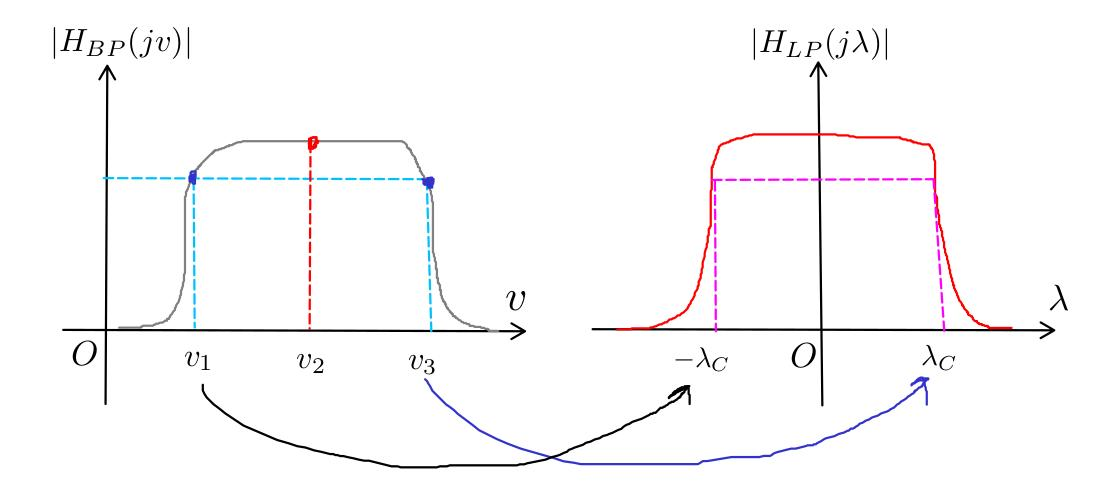
\includegraphics[width=0.8\textwidth]{27.jpg}
	\caption{Designing digital BP filter}			\label{fig:re2}
		\end{figure}
Do tài liệu tham khảo gốc viết rất mơ hồ về thuật toán thiết kế bộ lọc BP (mình không hiểu cách chứng minh công thức từ đâu ra), nên ta công nhận các kết quả sau:
\\ Với $v_{1},v_{3}$ là tần số cắt ở hai phía của bộ lọc BP số, và $v_{2}$ là \textbf{tần số có dạng trung bình hình học} ta có:
$$\tan^2{\left(\frac{\pi v_{2}}{2}\right)}=\tan^2{\left(\frac{\pi v_{1}}{2}\right)}\tan^2{\left(\frac{\pi v_{3}}{2}\right)}$$
$$D=\lambda_{C}\cot{\left(\frac{\pi}{2}(v_{3}-v_{1})\right)}$$

\end{frame}
\begin{frame}{Thiết kế bộ lọc số}
	$$E=\frac{2\cos{\left(\frac{\pi}{2}(v_{3}+v_{1})\right)}}{\cos{\left(\frac{\pi}{2}(v_{3}-v_{1})\right)}}$$
	$$\frac{\lambda}{D}=\frac{\cos(\pi v_{2})-\cos(\pi v)}{\sin(\pi v)}$$
	Đương nhiên, vì chúng ta muốn ánh xạ sang bộ lọc LP tương tự có \textbf{tần số cắt chuẩn hóa}, nên $\lambda_{C}=1$ (rad/s).
\\	Sau khi đã thiết kế bộ lọc tương tự chuẩn hóa $H_{LP,N}(p)$, ta đổi biến:
	$$p=D\frac{1-Ez^{-1}+z^{-2}}{1-z^{-2}}$$
Và thu được hàm truyền của bộ lọc số $H_{BP}(z)$ tương ứng.
	\end{frame}
\begin{frame}{Thiết kế bộ lọc số}
\begin{block}{Thuật toán thiết kế bộ lọc BP}
	\begin{enumerate}
		\item[1] Chuyển toàn bộ tần số $F$ ở miền số về các tần số số $v$ tương ứng theo quy chuẩn Matlab.
		\item[2] Xác định $v_{1}$, $v_{3}$, tính $v_{2}$, $D$, $E$, theo công thức trên.

			$$\alert{\tan^2{\left(\frac{\pi v_{2}}{2}\right)}=\tan^2{\left(\frac{\pi v_{1}}{2}\right)}\tan^2{\left(\frac{\pi v_{3}}{2}\right)}}$$
$$D=\lambda_{C}\cot{\left(\frac{\pi}{2}(v_{3}-v_{1})\right)}$$
	$$E=\frac{2\cos{\left(\frac{\pi}{2}(v_{3}+v_{1})\right)}}{\cos{\left(\frac{\pi}{2}(v_{3}-v_{1})\right)}}$$
\item[3] Ánh xạ từng tần số trong miền số $v\to\lambda$:
	$$\frac{\lambda}{D}=\frac{\cos(\pi v_{2})-\cos(\pi v)}{\sin(\pi v)}$$
\item[4] Thiết kế bộ lọc LP chuẩn hóa $H_{LP,N}(p)$ theo các thông số trên.
\item[5] Đổi biến:
$$p=D\frac{1-Ez^{-1}+z^{-2}}{1-z^{-2}}$$
Và ta thu được hàm truyền của bộ lọc BP số cần tìm.

	\end{enumerate}
	\end{block}
\end{frame}
\begin{frame}{Thiết kế bộ lọc số}
Ví dụ: thiết kế bộ lọc số có đặc tả sau biết $F_{sam}=2$ (kHz);
$$300<F<400\text{ (Hz)};\quad A<3\;(\text{dB})$$
$$F<200\text{ (Hz)},F>500\text{ (Hz)};\quad A>18\;(\text{dB})$$
Ta chọn bộ lọc Butterworth để thiết kế, hiển nhiên ta thấy:
$$F_{N}=1\text{ (kHz) }$$
Suy ra: $$v_{1}=0.3;v_{3}=0.4;v_{S1}=0.2;v_{S3}=0.5$$
Ta xác định tần số số $v_{2}$:
$$\tan^2{\left(\frac{\pi v_{2}}{2}\right)}=\tan^2{\left(\frac{\pi v_{1}}{2}\right)}\tan^2{\left(\frac{\pi v_{3}}{2}\right)}\Rightarrow v_{2}=0.3479$$
Với \alert{$\lambda_{C}=1$ (rad/s)}, ta tính $D$ và $E$:

$$D=\lambda_{C}\cot{\left(\frac{\pi}{2}(v_{3}-v_{1})\right)}=6.3137$$
	$$E=\frac{2\cos{\left(\frac{\pi}{2}(v_{3}+v_{1})\right)}}{\cos{\left(\frac{\pi}{2}(v_{3}-v_{1})\right)}}=0.9192$$
	Sử dụng công thức để ánh xạ các tần số dừng $v_{S}$ tương ứng:
	$$\frac{\lambda}{D}=\frac{\cos(\pi v_{2})-\cos(\pi v)}{\sin(\pi v)}\Rightarrow \lambda_{S1}=-3.7504;\lambda_{S3}=2.903$$
\end{frame}
\begin{frame}{Thiết kế bộ lọc số}
Để đảm bảo đặc tả thiết kế, ta chọn $\lambda_{S}$ sao cho bậc $N$ của bộ lọc cao nhất có thể.
\\ Vậy ta thiết kế bộ lọc LP Butterworth chuẩn hóa thỏa mãn đặc tả sau: $\lambda_{C}=1$, $\lambda_{S}=2.903$, $A_{P}=3$, $A_{S}=18$.
\\ Sử dụng phương pháp thiết kế đã được đề cập ở trên, ta thu được hàm truyền:
$$H_{LP,N}(p)=\frac{1}{p^2+1.41589p+1}$$
Đổi biến:
$$p=D\frac{1-Ez^{-1}+z^{-2}}{1-z^{-2}}=6.3137\frac{1-0.9192z^{-1}+z^{-2}}{1-z^{-2}}$$
Ta thu được hàm truyền $H_{BP}(z)$ của bộ lọc số cần tìm.
\end{frame}
\begin{frame}{Thiết kế bộ lọc số}
\begin{itemize}
	\item[-] Thiết kế bộ lọc HP
\end{itemize}
\begin{figure}[h]
	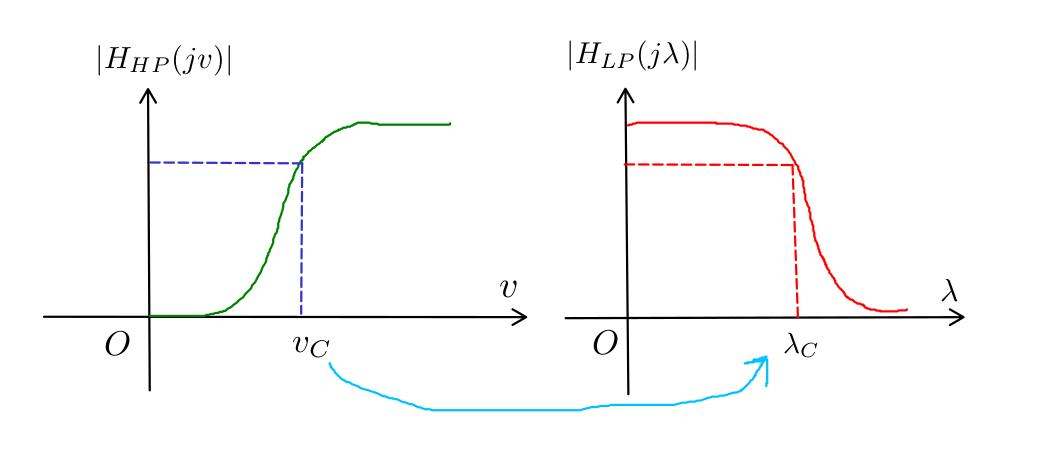
\includegraphics[width=0.8\textwidth]{28.jpg}
	\caption{Designing digital HP filter}			\label{fig:re2}
		\end{figure}
		Phép ánh xạ từ bộ lọc HP số sang LP tương tự chuẩn hóa với tần số cắt $\lambda_{C}=1$ (rad/s), hoàn toàn ngược với công thức thiết kế bộ lọc LP số.
		$$p=C\frac{1+z^{-1}}{1-z^{-1}}$$
		$$\lambda=C\cot{\left(\frac{\pi v}{2}\right)}\Rightarrow C=\lambda\tan{\left(\frac{\pi v}{2}\right)}$$
		Tương tự như trên, ta chọn $\lambda_{C}=1$ (rad/s) và thu được thuật toán thiết kế sau.
\end{frame}
\begin{frame}{Thiết kế bộ lọc số}
\begin{block}{Thuật toán thiết kế bộ lọc HP số}
	\begin{enumerate}
	\item[1] Chuyển các tần số trong miền số về các tần số số $v$:
		$$\alert{v=\frac{F}{F_{N}}}$$
	\item[2] Xác định tần số cắt số $v_{C}$, và tính hằng số $C$ theo công thức:
$$\alert{C=\tan{\left(\frac{\pi v_{C}}{2}\right)}}$$
\item[3] Ánh xạ từng tần số trong miền số sang miền tương tự với hằng số $C$ đã chọn ở trên:
	$$\alert{\lambda=C\cot{\left(\frac{\pi v}{2}\right)}}$$
\item[4] Thiết kế bộ lọc thông thấp chuẩn hóa $H_{LP,N}(p)$ với dữ kiện trên.
\item[5] Đổi biến:
	$$p=C\frac{1+z^{-1}}{1-z^{-1}}$$
	 Ta thu được hàm truyền của bộ lọc số $H_{LP}(z)$ cần tìm.
	\end{enumerate}
	\end{block}

\end{frame}
\begin{frame}{Thiết kế bộ lọc số}
Ví dụ: thiết kế bộ lọc số HP thỏa mãn đặc tả sau, biết $F_{sam}=50$ (kHz):
$$0<F<5\text{ (kHz)};\quad A>20\;(\text{dB})$$
$$F>10\text{ (kHz)};\quad 0<A<2.5\;(\text{dB})$$
Ta xác định tần số Nyquist: $$F_{N}=\frac{F_{sam}}{2}=25\text{ (kHz) }$$
Ta chọn bộ lọc Chebyshev và xác định các giá trị tần số số tương ứng:
$$v=\frac{F}{F_{N}}\Rightarrow v_{S}=0.2;v_{P}=0.4$$
Ta tính hằng số C: 
$$\alert{C=\tan{\left(\frac{\pi v_{C}}{2}\right)}}=0.7625$$
Ánh xạ tần số số sang miền tương tự:
$$\alert{\lambda=C\cot{\left(\frac{\pi v}{2}\right)}}\Rightarrow \lambda_{C}=1,\lambda_{S}=2.346$$
Ta xác định hàm truyền $H_{LP,N}(p)$ với đặc tả $\lambda_{C}=1,\lambda_{S}=2.346,r=2.5,A_{S}=20$:
$$H_{N,LP}(p)=\frac{0.2833}{p^3+0.6598p^2+0.9677p+0.2833}$$
\end{frame}
\begin{frame}{Thiết kế bộ lọc số}
Đổi biến:

	$$p=C\frac{1+z^{-1}}{1-z^{-1}}=0.7625\frac{1+z^{-1}}{1-z^{-1}}$$
Ta thu được hàm truyền của bộ lọc HP số cần tìm.
\end{frame}
\begin{frame}[fragile]{Thiết kế bộ lọc số}
\subsection{Thực hành}
\begin{itemize}
	\item Thực hành
\end{itemize}
Tương tự như phần Thực hành của bộ lọc tương tự, ta cũng dùng phần mềm mô phỏng tính toán để thiết kế các bộ lọc số.
\begin{verbatim}
Fp=...;Fs=...;Ap=...;As=...;Fsam=...; % LP filter
Fny=Fsam/2;
vp=Fp/Fny;vs=Fs/Fny;
[n vc]=buttord(vp,vs,Ap,As) % Butterworth filter
[b a]=butter(n,vc)
[n vc]=cheby1(vp,vs,Ap,As) % Chebyshev filter
[b a]=cheb1ord(n,Ap,vc)
freqz(b,a) % Plot frequency response
zplane(b,a) % Plot Z-plane to display zeros and poles
impz(b,a) % Display impulse response of system
\end{verbatim}
Đối với bộ lọc HP, cú pháp của Octave và Matlab có một chút khác biệt, ở đây mình thiết kế bằng Octave:
\begin{verbatim}
	[n vc]=buttord(vp,vs,Ap,As) % Doesn't have 'high' parameter
	[b a]=butter(n,vc,'high') % Has 'high' parameter
\end{verbatim}
Với bộ lọc BP, ta khởi tạo 2 mảng:
\begin{verbatim}
vp=[starting_point,ending_point];vs=[starting_point,ending_point];
[n vc]=buttord(vp,vs,Ap,As) % Doesn't have 'bandpass' parameter
[b a]=butter(n,vc,'bandpass') % Has 'bandpass' parameter
\end{verbatim}
Với bộ lọc BS, ta chỉ cần thay \verb|'bandpass'| thành \verb|'stop'| là xong.
\end{frame}
\end{document}
